\RequirePackage{plautopatch}
% \documentclass[report,paper=a4, fontsize=12pt, line_length=16cm, number_of_lines=33]{jlreq}
% \usepackage[haranoaji,deluxe]{luatexja-preset}
% \usepackage{amsmath,amssymb}
% \usepackage{libertinus}

\documentclass[report,paper=a4, fontsize=12pt, line_length=16cm, number_of_lines=33,dvipdfmx]{jlreq}
\usepackage{jlreq-deluxe}
\usepackage{amsmath,amssymb}
\usepackage{stix2}
\renewcommand{\bfdefault}{bx}
% \usepackage{libertine}
% \usepackage{libertinust1math}
% \usepackage[T1]{fontenc}
% \usepackage{mlmodern}
% \usepackage[T1]{fontenc}
% \usepackage{tgtermes,tgheros,tgcursor}
% \renewcommand{\bfdefault}{bx}
% \usepackage[libertine]{newtxmath}

%% Fonts
%\usepackage{lmodern}
%\usepackage[T1]{fontenc}

\usepackage{tikz}

\usepackage{hyperref}
\hypersetup{colorlinks=true,linkcolor=blue,citecolor=blue}

\usepackage{graphicx}
\graphicspath{{fig/}}

\usepackage{physics}
\usepackage{color}

\usepackage{tcolorbox}
\tcbuselibrary{breakable, skins, theorems}
%\usepackage{cleveref}

% font warningを出さないため
% \DeclareFontShape{JY2}{hgt}{b}{n}{<->ssub*hgt/bx/n}{}
% \DeclareFontShape{JY2}{hgt}{m}{it}{<->ssub*hgt/m/n}{}
% \DeclareFontShape{JT2}{hgt}{b}{n}{<->ssub*hgt/bx/n}{}
% \DeclareFontShape{JT2}{hgt}{m}{it}{<->ssub*hgt/m/n}{}

\newcommand{\preface}[1]{\section*{#1}}

\newenvironment{myquote}{\begin{tcolorbox}[
  colback = blue!5, after = \noindent] }{\end{tcolorbox}}
\newenvironment{important}{\begin{tcolorbox}[
  colback = white,
  colframe = red!35,
  boxrule = 2mm,
  fonttitle = \bfseries,
  after = \noindent] }{\end{tcolorbox}}
\newenvironment{mycite}{\\ \qquad \textbullet\ }{\\}

\newtcolorbox{emphasize}[1][]{
  colback=orange!7,
  colframe=orange!80!red,
  coltitle=white,
  title={#1},
  fonttitle=\sffamily \bfseries, 
  sharp corners,
  boxrule=0.5mm
}
\newtcolorbox{proposition}[1][]{
  colback=white,
  colframe=green!40,
  coltitle=black,
  title={#1},
  fonttitle=\sffamily \bfseries, 
  sharp corners,
  boxrule=0.5mm
}

\newcommand{\underrem}[2]{
    {\color{red} \underbrace{\color{black} {#1}}_{\text{#2}}
    }
}

\newcommand{\overrem}[2]{
    {\color{red} \overbrace{\color{black} {#1}}^{\text{#2}}
    }
}

\newcommand{\qed}{■}
\newcommand{\kyou}[1]{{\sffamily \bfseries #1}}

\numberwithin{equation}{chapter}
%%%%%%%%%%%%%%%%%%%%%%%%%%%%%%%%%%%%%%%%%%%%%%%%%%%%%%%%%%%%%%%%%%%%%%
%                          often used macro
\newcommand{\del}{\partial}
\newcommand{\Cb}{\mathbb{C}}
\newcommand{\Zb}{\mathbb{Z}}
\newcommand{\CP}{\Cb \mathrm{P}}
%\newcommand{\strong}[1]{{\sffamily \gtfamily \bfseries #1}}
\newcommand{\Ztwo}{\mbox{$\mathbb{Z}_{2}$}}
\newcommand{\Hh}{\widehat{H}}
\newcommand{\Uh}{\widehat{U}}
\newcommand{\Vh}{\widehat{V}}
\newcommand{\Jh}{\widehat{J}}
\newcommand{\Qh}{\widehat{Q}}
\newcommand{\Oh}{\widehat{\mathcal{O}}}
\newcommand{\Gh}{\widehat{G}}
\newcommand{\ah}{\hat{a}}
\newcommand{\bh}{\hat{b}}
\newcommand{\Ocal}{\mathcal{O}}
\newcommand{\Ocalh}{\widehat{\mathcal{O}}}
\newcommand{\Ncal}{\mathcal{N}}
\newcommand{\U}{\mbox{U}}
\newcommand{\ZIsing}{Z_{\mathrm{Ising}}}
\newcommand{\Zgauged}{Z_{\mathrm{Ising}/\Zb_2}}
\newcommand{\deltamod}[1]{\delta^{\mathrm{mod} \ 2}_{#1}}
\newcommand{\Kt}{\widetilde{K}}
\newcommand{\link}[1]{\expval{#1}}
\newcommand{\plaq}[1]{\expval{#1}}

\newcommand{\Ising}{\mbox{Ising}}
\newcommand{\gIsing}{\mbox{Ising$/\Zb_2$}}

\newcommand{\Tcal}{\mathcal{T}}
\newcommand{\Lambdah}{\widehat{\Lambda}}

\title{一般化対称性について}
\author{山口 哲}
\date{\today}
\begin{document}
\maketitle
\tableofcontents

\preface{まえがき}

このノートは2023年10月に東京大学駒場で行った集中講義のノートです。集中講義の機会をくださり、有益な議論をしてくださった東京大学駒場素粒子論研究室の皆様、集中講義の参加者の皆様に感謝いたします。

\chapter{導入}
\section{対称性とは?}

この講義では、対称性の一般化について取り扱います。一般化に行くまえに普通の対称性について質問したいと思います。(場の理論において)対称性とは何でしょうか?考えてみてください。この質問は哲学的に聞こえるかもしれませんが、もっと具体的なもので、例えばみなさんが授業や教科書でどう習ったか、あるいは授業どう教えているかというものです。

答えはいろいろあると思います。ここでは、その中の3つをとりあえず書いてみます。この中に皆さんの考えた答えはあるでしょうか?
\begin{itemize}
  \item[①] 場を$\phi$、作用を$S(\phi)$とします。対称性とは変換$\phi\to\phi'$であって$S(\phi')=S(\phi)$となるものです。
  \item[②] Hamiltonianを$\Hh$とします。対称性とはUnitary演算子$\Uh$であって、Hamiltonianと交換する、つまり$\Hh \Uh =\Uh \Hh$となるものです。
  \item[③] 余次元1のトポロジカル欠陥で群構造を持つもの。  
\end{itemize}
①は、一番人気がある答えで、多くの人がこれを思い浮かべたと思います。②も量子力学では良く出てくる説明で、これを思い浮かべなかった人も言われてみれば納得してもらえると思います。③は異質ですね。これは普通の教科書には載っていないです。意味が分からなかったとしてもひとまず気にしないでください。③はこの後この講義で時間をかけて説明したいことの一つです。これが①や②と同じレベルで納得してもらえれば、この講義の目的の目的の半分くらいは達成したと言えます。

さて、①や②のような分かりやすい言い方があるのに、なぜ③のような難しい言い方を知らないといけないのでしょうか。実は①や②には次のように「大域的である」という共通の不満があるのです。
\begin{itemize}
  \item[①] 変換は時空全体で一斉に変換してみることが必要になります。宇宙を考えているなら、宇宙の始まりから未来まで、ほぼ真空のところや星の中から宇宙の果てまで一斉に変換して作用が不変か?という問でしか対称性の存在を記述できていません。
  \item[②] こちらは時間方向は考えなくても良いですが、$\Hh$も$\Uh$も空間全体に広がる巨大な演算子です。しかも系のサイズによって(Hilbert空間の次元も含めて)変わります。 両方とも局所的なものの集まりなので、局所的な性質を見れば全体をいっぺんに考えなくても良いはずなのですが、②の言い方では全体でしか考えられていません。
\end{itemize}
つまり、対称性の記述としては
\begin{emphasize}
  (大域的対称性であっても)局所的な記述が望ましい。
\end{emphasize}
ということになります。

この不満は最近になって降って湧いたわけではなく、昔からありました。そしてその解決もされています。それが、最初の質問に対する4番目の答えです。
\begin{itemize}
  \item[④] 対称性とは、(連続対称性の無限小変換の場合には)カレント$J^{\mu}(x)$であって、$\del_{\mu}J^{\mu}(x)=0$を満たすことである。
\end{itemize}
最初の問でこれを思い浮かべられた方もおられたかも知れません。また、言われてみれば皆さん納得されると思います。この記述は完全に局所的で理想通りです。場の理論で対称性を用いて様々な性質を導くときに、この記述は大変便利で、欠くことができないものです。

④の答えは非常に良いものでしたが、難点は連続対称性の無限小変換に限られることです。例えば離散的対称性の場合にはカレントは存在しませんから、④の記述はありません。実は離散的な対称性の場合にも適用できる局所的な記述が③です。
\begin{emphasize}
  ③のトポロジカル欠陥は対称性の局所的な記述を与える。  
\end{emphasize}
このような理由で③の見方は、普通の対称性に対しても有用です。

\section{対称性の使い方の例}

この後、対称性の一般化について説明していくわけですが、対称性を一般化しても有用であるということを説明するために、対称性の使い方の一つをについて説明します。これは簡単な例ですが、量子力学の教科書にはあまり書いてないと思います。

次のような命題が成り立ちます。
\begin{proposition}[命題]
$\Uh,\Vh$をユニタリー演算子で、Hamiltonian $\Hh$と可換とします(つまり、②の見方での対称性です。)。そして
\begin{align}
  \Uh \Vh = a \Vh \Uh,\quad (a \text{はc数},\ a\ne 1)
  \label{anomaly}
\end{align}  
とします。このとき、\kyou{すべてのエネルギー準位(特に基底状態)は縮退しています。}
\end{proposition}
これは、場の理論の文脈では 't Hooft アノマリー整合条件と呼ばれているものの一例です。$a$がこの例での 't Hooft アノマリーになります。おそらく、普通に場の理論でアノマリーを勉強された方には、そのアノマリーとこの$a$がどう関係があるか分からないと思います。大事なことではあるのですが、この講義の主題とは外れるのと、知らなくてもこの命題だけで理解できるので、その説明は省略します。

\kyou{証明} 証明を与えます。背理法で証明します。つまり、縮退していないエネルギー固有状態$\ket{\psi},\ \Hh \ket{\psi}=E\ket{\psi}$があると仮定します。このとき$\Uh\ket{\psi}$がエネルギー$E$の固有状態であることが、次のようにして分かります。
\begin{align}
  \Hh \Uh \ket{\psi} =\Uh \Hh \ket{\psi}
  =E\Uh \ket{\psi}.
\end{align}
さらに縮退が無いことがら$\Uh \ket{\psi}\propto \ket{\psi}$なので、次のように表すことができます。
\begin{align}
  \Uh \ket{\psi}=u\ket{\psi},\ u\in \Cb,\ |u|=1.
\end{align}
$\Vh$に関しても同様です。
\begin{align}
  \Vh \ket{\psi}=v\ket{\psi},\ v \in \Cb,\ |v|=1.
\end{align}
これらを用いると
\begin{align}
  \Uh \Vh \ket{\psi}=uv\ket{\psi}
\end{align}
という関係を得ます。ところが、\eqref{anomaly}の関係を用いると、全く同じベクトルが
\begin{align}
  \Uh \Vh \ket{\psi}=a\Vh \Uh \ket{\psi}=a u v \ket{\psi}
\end{align}
とも書けます。ここから
\begin{align}
  auv\ket{\psi}=uv\ket{\psi}
\end{align}
という関係式を得ます。$uv\ket{\psi}\ne 0$ですから、この式は$a\ne 1$に矛盾します。\qed 

ここで考えてみたいことは、\kyou{$\Uh,\Vh$ がユニタリーでなかったらどうなるか?}ということです。この場合、$\Uh,\Vh$ ユニタリーではありませんから、従来の意味での対称性ではありません。しかし、証明を見てもらって分かるように、ユニタリー性を用いているところは$uv\ket{\psi}\ne 0$の部分のみです。ですから、この場合も命題を少し修正することで成り立ちます。このようにして「(従来の意味では)対称性でないもの」を対称性と同じように用いて理論を調べることができるわけです。このように従来の意味では対称性でないが、対称性と同様な使い方ができるものを「一般化対称性」と呼んでいろいろ調べようというのがここでやりたいことです。

上の証明を見てもらって分かるように、対称性の最も重要な性質はHamiltonianと交換するということです。これをゆるめてしまうと、対称性と同じように用いることは、なかなか難しくなります。したがって、ここではこの条件はゆるめないことにします。一方、ユニタリーのような条件はゆるめても、そこそこ使えるものになります。これを「一般化対称性」と呼んで、いろいろ調べよう、というのがこの講義の目的です。ユニタリーでないがHamiltonianと交換する演算子は場の理論の文脈では「非可逆対称性」と呼ばれます。\footnote{非可逆対称性という名前の由来については、少々複雑です。ちゃんと説明するためには場の理論でのトポロジカル欠陥について知ってもらう必要があります。ここでは、\kyou{非可逆対称性という名前だけれど$\Uh$という演算子が非可逆とは限らない}、ということだけ注意しておきます。}

\section{いくつかの注意}\label{sec:remarks}
ここでは、通常のセミナーなどでは説明が省略されることが多いけれど、注意が必要なことについて説明します。

一つは、Euclideanの定式化についてです。この講義も含めて、セミナーや論文などでは場の理論をEuclid形式で取り扱うことがよくあります。これは、「Euclid形式の場の理論」という、教科書に出てくる場の理論と異なる理論を考えているのではないことに注意してください。理論は教科書に出てくる場の理論と同じものを取り扱っています。異なるのは定式化の仕方とか計算しやすい量です。例えば正準分配関数はEuclid形式で取り扱いやすい量の一つです。これは
\begin{align}
  \Tr e^{-\beta \Hh} = \int D\phi e^{-S_{E}(\phi)}
\end{align}
のように表すことができます。ここで、$S_{E}(\phi)$は虚時間方向を長さ$\beta$の円周にしたときのEuclid化した作用です。他にも、$\Ocalh_1(x_1),\dots, \Ocalh_K(x_K)$をすべて同時刻の別々の点に置かれた局所演算子としたとき、
\begin{align}
  \expval{\Ocalh_1(x_1) \dots \Ocalh_K(x_K)}{0}
  =\frac{1}{Z}\int D\phi e^{-S_{E}(\phi)} \Ocal_1(x_1) \dots \Ocal_K(x_K),\quad 
  Z:=\int D\phi e^{-S_{E}(\phi)}.
\end{align}
と表すことができます。このとき$S_E(\phi)$はEuclid化した作用です。他にも様々な量がEuclid形式を用いて計算することができます。この講義でもEuclid形式用いて様々な場の理論の性質を考えることになります。

もう一つは演算子関係式についてです。例えば、この講義でも\kyou{量子論で}
\begin{align}
  \del_{\mu}J^{\mu}(x)=0\label{egoperatorrelation}
\end{align}
というような式を書くことがあります。これは古典論であれば、運動方程式を満たす場の配位において、このような関係式を満たすということですが、量子論においてはどうでしょうか?一つは演算子形式の場の理論で$\Jh^\mu(x)$が上の関係式を満たすということです。この講義で主に用いるのは、もう少し広い応用ができる見方で、相関関数の間の関係式と見ることです。これは、
\begin{align}
  \expval{\del_{\mu}J^{\mu}(x)\cdots}=0,&\quad(\text{$\cdots$は任意の局所演算子や非局所演算子の挿入。}\notag\\&\text{ただし$x$は$\cdots$の挿入されている点とは異なる。})
\end{align}
というのを省略して書いたのが式\eqref{egoperatorrelation}ということです。問題は「ただし…」のところは文脈によって色々変わるところです。この講義では分かりにくそうな場合はなるべく補足するようにはしますが、もし分からなければ聞いてください。

他によく使う例として
\begin{align}
  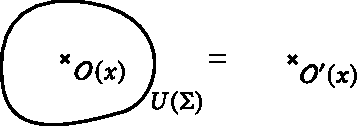
\includegraphics{EgWTid.pdf}
\end{align}
というようなものがあります。これは$x$は時空の点で$\Ocal(x),\Ocal'(x)$は局所演算子、$\Sigma$は余次元1の面で$U(\Sigma)$は$\Sigma$に局在した演算子(欠陥)です。この「式」の意味は
\begin{align}
  \expval{U(\Sigma)\Ocal(x)\cdots}=\expval{\Ocal'(x)\cdots},\qquad&(\text{$\cdots$は両辺で共通の任意の演算子の挿入。 }\notag \\
  &\text{ただし、$\cdots$は$\Sigma$の内側には挿入されていない。})
\end{align}
という意味です。

\chapter{対称性とトポロジカル欠陥}\label{sec:symmetrydefect}

この章の目標は、前章で紹介した対称性の③の見方「対称性とは余次元1のトポロジカル欠陥で群構造を持つもの」ということを納得してもらうことです。まず、欠陥という概念を導入します。そして対称性がトポロジカル欠陥であることを様々な観点から説明します。一旦それを納得してもらえば、対称性の一般化はすんなりと納得してもらえると思います。

\section{欠陥}\label{sec:defect}

まず、欠陥を定義します。
\begin{emphasize}
  場の理論において\kyou{欠陥(defect)}とは、\kyou{時空の中で他の部分と性質が異なる部分}のことを言います。 ただし、局所性を満たすものとします。 
\end{emphasize}

補足の説明をします。性質が異なるというのは、例えばLagrangian密度がそこだけ異なるとか、余分な自由度がそこにあるとか、格子の理論なら、そこだけ格子の構造が異なるとか、そういうものです。

局所性というのは、性質が異なるとしても非局所的な相互作用はないということです。言い換えれば、欠陥の上の離れた2点が直接相互作用をすることは無いようなものです。格子理論で考える場合には、連続極限をとったときに局所性を満たすようなものなら、それは局所性を満たす欠陥であると言うことにします。

別の言い方をすると、欠陥とは(広い意味での)演算子であるということもできます。

次に2つの言葉を導入します。まず、欠陥の\kyou{次元}とは、性質の異なる部分の次元を言います。例えば時空の中で1点が他の部分と異なるなら、その次元は1です。\kyou{余次元(codimension)}とは、時空の次元を$d$、欠陥の次元を$p$としたときに、$d-p$のことを言います。欠陥の性質は余次元によって共通な場合もあるので、この言葉を導入するのが便利です。これは単に言葉遣いの問題なのですが、余次元0の欠陥、つまりある領域にわたって性質が違うようなものは欠陥とは呼ばないことにします。

代表的な欠陥の例を2つ挙げます。局所演算子は0次元の欠陥です。別の言い方をするなら、局所演算子とは時空の1点にある欠陥の別名です。\footnote{局所演算子はLagrangianに出てくる場の微分やそれらの積で書けているものに限りません。}もう一つの例はゲージ理論のWilsonループ$\Tr P \exp\left(i\oint A\right)$です。Wilsonループは1次元の欠陥の例です。

欠陥について一つ注意することは、欠陥は動的な物体、例えばソリトンなどではないということです。動的な物体は運動方程式などにしたがって運動しますが、欠陥はその部分の物理法則を手で変えるようなものです。欠陥の形などは手で決めます。ややこしいことに文献によってはソリトンのことを欠陥と呼んでいるものもあるので注意が必要です。

\section{対称性とトポロジカル欠陥その1}

ここから対称性とトポロジカル欠陥の関係について見ていきます。

まず、\kyou{トポロジカル欠陥(topological defect)}とは、欠陥のうちでトポロジーを変えない連続変形で値を変えないもののことを言います。\footnote{これも不幸な用語の行き違いなのですが、トポロジー的に守られて安定なソリトンのことをトポロジカル欠陥と呼ぶ文献もあります。これはこの講義でのトポロジカル欠陥とは違うものです。}
絵を使った式で書くなら
\begin{align}
  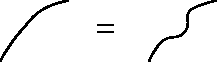
\includegraphics{topologicaldefect.pdf}
\end{align}
のようになります。この式も\ref{sec:remarks}節で述べた演算子関係式の書き方を使っています。つまり、左辺と右辺は他に任意の共通の演算子が挿入されている期待値です。ただし、欠陥を変形している部分には演算子は挿入されていません。

ここから考えていきたいことは、みなさんが納得しているはずの対称性の見方②$\Hh \Uh = \Uh \Hh$、および④$\del_{\mu}J^{\mu}=0$から始めて、③トポロジカル欠陥の見方ができることを示すことです。

\subsection{ユニタリー演算子とトポロジカル欠陥}

$d$次元の場の理論の演算子形式の定式化から始めることにします。簡単のために$\U (1)$対称性の場合を考えます。時刻$0$で対称性のユニタリー演算子は変換のパラメーターを$\alpha$として、
\begin{align}
  \Uh=e^{i\alpha \Qh},\qquad
  \Qh:=\int_{t=0,\ \text{空間}}d^{d-1}x \Jh^0. 
\end{align}
$\Jh^{0}$はカレント$\Jh^{\mu},\ \mu=0,\dots,d-1$の時間方向成分、つまり電荷密度です。$\Qh$の定義は空間が有限(周期境界条件など)の場合には良いですが、無限の場合には積分が定義されるかどうかが問題となります。実は自発的対称性の破れが起こっている場合には、この積分は収束しません。自発的対称性の破れについては、教科書\cite{Kugo2}が詳しいです。ここではひとまず定義されている場合を考えることにします。

Euclideanの定式化を使うために、
\begin{align}
  \Jh^{d}:=i\Jh^{0}
\end{align}
を定義します。\footnote{これを見て分かるように、Euclideanの定式化ではHermit共役には注意する必要があります。} これを用いると
\begin{align}
  \Qh = -i \int_{t=0,\ \text{空間}}d^{d-1}x \Jh^{d}
\end{align}
と書けます。

Euclid時間(虚時間)を$\tau$として、Euclid時間発展について考えます。$\Oh$を時刻$0$での演算子として、Heisenberg演算子のような役割をする演算子$\Oh(\tau)$を
\begin{align}
  \Oh(\tau):=e^{\tau \Hh}\Oh e^{-\tau \Hh}
\end{align}
と定義します。\footnote{本当のHeisenberg演算子と区別するために記号を変える方が良いのかもしれませんが、煩雑になるのでやめておきます。本物のHeisenberg演算子とは違うものであることに注意してください。また、ここで定義したEuclideanのHeisenberg演算子のようなものは取り扱いには注意が必要です。$e^{|\tau| \Hh}$という高エネルギーのところが大きく効いてくる演算子が入っているからです。ただし、これらの演算子の時間順序積の真空期待値などはちゃんと定義されます。Euclideanの経路積分形式と演算子形式をつなぐときに考えると便利な書き方だと思うと良いと思います。} こうすると、例えばカレントの保存則$\del_{\mu}\Jh^{\mu}(x^0,\vec{x})=0,\ \mu=0,\dots, d-1$は、$x^d:=\tau$として
\begin{align}
  \del_{\mu}\Jh^{\mu}(\vec{x},x^{d})=0,\ \mu=1,\dots,d
\end{align}
と書くことができます。また、$\Uh \Hh = \Hh \Uh$ですから
\begin{align}
  \Uh(\tau)=\Uh
  \label{conservation}
\end{align}
となります。

式\eqref{conservation}をEuclidean経路積分形式での期待値の関係式に書くと
\begin{align}
  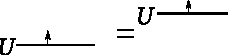
\includegraphics{conservation.pdf}\label{coservationfig}
\end{align}
のようになります。ここで矢印で向きを表しています。

$U$は時間一定面で他の部分とは異なっているので、余次元1の欠陥です。式\eqref{coservationfig}は、$U$を時間方向にずらしても値を変えないことを示しています。これから、$U$がトポロジカル欠陥であることを示します。

これから書くのはEuclidean経路積分形式での演算子関係式です。余次元1の向きのついた部分多様体を$M$として
\begin{align}
  U(M):=e^{i\alpha \Qh(M)},\quad
  Q(M):=-i\int_{M}dS_{\mu}J^{\mu}
\end{align}
とします。\footnote{$U(M)$の定義の中に$\exp$があって、同じ点での演算子の積が入っています。一般には、ここで発散があったり、繰り込みが必要だったりして微妙なことが起こるのですが、ここではひとまず説明のために無視します。正しい取り扱いは、次節でやる背景ゲージ場とそのゲージ変換を用いる方法です。}$\int_{M}dS_{\mu}$は電磁気の授業などで出てきた面積分です。

この$U(M)$がトポロジカルであることは次のようにして示します。ある領域$D$があって、$\del D=M\cup (-M')$とします。ただし、$-M'$は$M'$の向きを反対にしたものです。こうするとGaussの定理を用いて
\begin{align}
  \int_{D}d^d x \del_{\mu}J^{\mu}
  =\int_{M}dS_{\mu}J^{\mu}-\int_{M'}dS_{\mu}J^{\mu}
\end{align}
を得ます。ここから
\begin{align}
  Q(M)=Q(M'),\qquad U(M)=U(M')
\end{align}
という式が成り立ちます。特に$M_1$と$M_2$がトポロジーを変えない連続変形で繋がっている場合には領域$D$で、$\del D=M_1\cup (-M_2)$となるものがとれますから、$U(M_1)=U(M_2)$となり、したがって$U$はトポロジカル欠陥ということが言えました。

ここまでで言えたことをまとめます。
\begin{emphasize}
  対称性があると対応するトポロジカル欠陥がある。それは、対称性の演算子$\Uh$を時間一定面だけでなく、曲がったところにも定義したものである。
\end{emphasize}
最初の方で、自発的対称性の破れがあるときには$\Uh$がうまく定義できないと言いました。しかし、これは定義しようとしている空間が無限であるところからくるものです。したがって、$M$が有限である場合には$U(M)$は自発的対称性の破れがあるかどうかにかかわらず定義でき、理論の解析に用いることができます。

\subsection{局所演算子への作用}

次に対称性の局所演算子への作用について考えてみます。場の理論の演算子形式では、局所演算子$\Oh(x)$変換は
\begin{align}
  \Uh \Oh(x) \Uh^{\dag}=\Oh'(x)
  \label{transformation0}
\end{align}
と書けます。\footnote{量子力学の教科書とは異なるconventionを用いています。場の理論の論文では、ここで用いるconventionの方が一般的です。}
$\Uh,\Uh^{\dag}$は$\Hh$と可換ですから、$\Uh$を少しだけ虚時間で未来に移動し、$\Uh^{\dag}$を少しだけ過去に移動することで
\begin{align}
  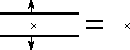
\includegraphics{transformation0.pdf}
\end{align}
という絵で表すことができます。別の言い方をすると式\eqref{transformation0}の左辺は、
\begin{align}
  T(\Uh(M_1)\Oh(x)\Uh(M_2))=T(\Uh(M)\Oh(x)),\quad
  M:=M_1 \cup (-M_2)
\end{align}
と表すことができます。$T()$は虚時間順序積を表します。さらに$\cdots$を$x$と同時刻にはない任意の演算子の挿入として\eqref{transformation0}より
\begin{align}
  \ev{T(\Uh(M)\Oh(x)\cdots)}{0}=\ev{T(\Oh'(x)\cdots)}{0}
\end{align}
という式が成り立ちます。この両辺に現れる量をEuclidean経路積分で表すことを想定して
\begin{align}
  \expval{U(M)\Ocal(x)\cdots}=\expval{\Ocal'(x)\cdots}
\end{align}
と書くのでした。さらにこれを略記して
\begin{align}
  U(M)\Ocal(x) = \Ocal'(x)
\end{align}
と書きます。$U(M)$はトポロジカルですから、連続変形して(変形後の面も同じ記号$M$で表すことにして)
\begin{align}
  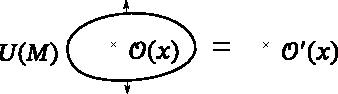
\includegraphics{transformation1.pdf}
\end{align}
という絵で書きます。これが、局所演算子の変換性をトポロジカル欠陥を用いて表したものになります。後で示すように、これはWard-Takahashi恒等式を有限変換の場合にも適用できる形にしたものと言うこともできます。

\section{対称性とトポロジカル欠陥その2}
ここでは、対称性とトポロジカル欠陥の関係を先程とは少し別の角度から見てみます。ここでは、通常のWard-Takahashi恒等式を①の描像から導くのと同様の方法を離散対称性の場合にも適用できるように有限変換で行います。つまり、大域的対称性であっても場所に依存する変換し、それによる作用の変化を見ます。

\subsection{分配関数と対称性欠陥}
$d$次元の場の理論を考えます。場を$\phi(x)$とし、作用を$S(\phi)$とします。この系に①の意味での大域的対称性があるとします。つまり、群$G$があり、$g\in G$に対して変換$\phi(x) \to \phi^g(x)$があって、$S(\phi^g)=S(\phi)$となるとします。$G$は連続的でも離散的でも良いです。

アイデアは、大域的対称性であっても場所に依存する変換、つまりゲージ変換をしてみることです。離散対称性でも適用できるように次のような変換を考えます。Euclidean時空の中の領域$D$をとり、変換
\begin{align}
  \phi'(x)=
  \begin{cases}
    \phi^g(x), & x\in D\\
    \phi(x), & x \notin D
  \end{cases}
  .\label{gaugetransf}
\end{align}
を考えます。つまり、領域$D$内では、$g$での変換を行い、$D$の外では変換しません。この変換を用いて分配関数を変形していきます。
\begin{align}
  Z&=\int D\phi e^{-S(\phi)}\notag\\
   &= \int D\phi' e^{-S(\phi')}\notag\\ 
   &= \int D\phi e^{-S_{D,g}(\phi)}.\label{derWT1}
\end{align}
この変形では、1行目から2行目は単に積分変数の文字を変えただけです。2行目から3行目へは変換\eqref{gaugetransf}を代入しました。簡単のため、この変換で積分測度$\int D\phi$は不変であることを仮定しました。また、$S_{D,g}(\phi):=S(\phi')$と定義しました。

さて、一般には変換で$S_{D,g}(\phi)\ne S(\phi)$です。どれくらい異なるかを考えてみましょう。まず、$D$の外部では$\phi(x)=\phi'(x)$ですから、同じです。一方、$D$の内部では$\phi\to \phi^g$が大域的対称性であることから、同じになることが分かります。つまり、\kyou{$S_{D,g}(\phi)$と$S(\phi)$は$M:=\del D$の部分でのみ異なることになります。} ですので、$M$に局在している演算子(欠陥)を
\begin{align}
  U_{g^{-1}}(M):=\exp(S(\phi)-S_{D,g}(\phi))
\end{align}
の挿入で定義することにします。すると\eqref{derWT1}から
\begin{align}
  Z=\int D\phi e^{-S(\phi)}U_{g^{-1}}(M)
\end{align}
を得ます。この両辺を$Z$で割ると
\begin{align}
  \expval{U_{g^{-1}}(M)}=1
\end{align}
という恒等式を得ます。これがWard-Takahashi恒等式の一種です。

$D$の外側に他の演算子(欠陥)がささっている場合も全く同様の変形ができて、次の恒等式を得ます。
\begin{align}
  \expval{U_{g^{-1}}(M)\cdots}=\expval{\cdots}
\end{align}
このような式を単に
\begin{align}
  U_{g^{-1}}(M)=1\quad (\text{ただし$M$の内側には他の演算子がささっていない})
\end{align}
と式で表したり、
\begin{align}
  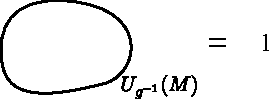
\includegraphics{EgWTid0.pdf}
\end{align}
と絵で表したりするのでした。

\subsection{演算子への作用}
この味方で演算子への作用を考えてみます。$\Ocal(x)$を局所演算子とし、それが$g\in G$で$\Ocal^{g}(x)$と変換するとします。

$D$の内部に$\Ocal(x)$を置き、その他の任意の演算子(欠陥)を$D$の外部に置きます。そして先程と同じように\eqref{gaugetransf}を考えます。すると
\begin{align}
  Z\expval{\Ocal(x)\cdots}
  =\int D\phi \Ocal(x)\cdots e^{-S(\phi)}
  =\int D\phi U_{g^{-1}}(M)\Ocal^{g}(x)\cdots e^{-S(\phi)}
\end{align}
という恒等式を得ます。これは
\begin{align}
  U_{g^{-1}}(M)\Ocal^{g}(x)=\Ocal(x)
\end{align}
と書くのでした。ここで、$\Ocal^{g}(x)$のことを$\Ocal(x)$と書き$g$のことを$g^{-1}$と書くことで
\begin{align}
  U_{g}(M)\Ocal(x)=\Ocal^{g}(x)
\end{align}
という恒等式を得ます。これは絵で
\begin{align}
  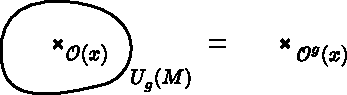
\includegraphics{EgWTid1.pdf}
\end{align}
というふうに表すこともできます。

$G$は群ですから、演算子への作用も表現になっています。ですから、表現行列を用いてWard-Takahashi恒等式を表しておくことも便利です。すべての局所演算子の基底を$\Ocal_{a}(x)$とすると、$\Ocal_{a}^{g}(x)$はこれらの線形結合で表すことができます。つまり$R(g)^{b}{}_{a}$を表現行列として
\begin{align}
  \Ocal^{g}_{a}(x)=\sum_{b}\Ocal_{b}(x)R(g)^{b}{}_{a}
\end{align}
と書くことができます。
これらすべてまとめて次のように言うことができます。
\begin{emphasize}
  離散的な群の場合も含めて、トポロジカル欠陥が対称性の局所的な記述を与える。この対称性を記述するトポロジカル欠陥を\kyou{対称性欠陥}と呼ぶ。Ward-Takahashi恒等式は
  \begin{align}
    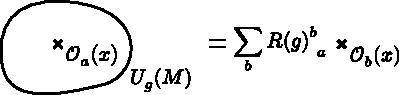
\includegraphics{EgWTid2.pdf}
  \end{align}
  と表せる。    
\end{emphasize}

\subsection{背景ゲージ場}
対称性を表すトポロジカル欠陥の便利な見方の一つは、背景ゲージ場を考えることです。結論から言うと、flatな背景ゲージ場の背景が対称性のトポロジカル欠陥の配位と同一視できます。それをこれから説明していきます。

簡単のため、連続対称性でアノマリーが無い場合を考えます。前節と同じ設定で、大域的対称性の背景ゲージ場$A$を入れた作用を$S(\phi,A)$とします。$A=0$のときに元の作用に戻るとします。つまり$S(\phi,A=0)=S(\phi)$とします。この背景ゲージ場の元での分配関数は
\begin{align}
  Z(A)=\int D\phi e^{-S(\phi,A)}
\end{align}
と表すことができます。

ここでゲージ変換について考えてみます。$A=0$のところから、前項で考えたゲージ変換\eqref{gaugetransf}をしてみます。このとき、$A\to A'$と変化します。ゲージ不変性は仮定しているので
\begin{align}
  Z(A=0)=Z(A')
\end{align}
となります。前項で議論したように、左辺は$M=\del D$に対称性欠陥が入った分配関数です。これがゲージ場$A'$が入っているのと同じということです。

$A'$は$A=0$から\eqref{gaugetransf}から得られたものですから、$A'$は$M$上だけでデルタ関数的に非0の値を持っています(図\ref{fig:localizedgaugefield}参照)。その値は$D$の中の点から外の点への経路で$M$と1回交わる経路を$C$として
\begin{align}
  P e^{i\int_{C}A'} = g
\end{align}
となるようになっています。また、もともと場の強さは$0$でしたから、ゲージ変換した後も$0$となります。このように場の強さが0となるゲージ場の配位を\kyou{flat}なゲージ場といいます。

\begin{figure}
  \centering
  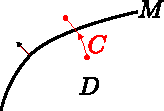
\includegraphics[width=6cm]{localizedgaugefield.pdf}
  \caption{対称性欠陥と背景ゲージ場の配位。$M$上にある対称性欠陥は$M$上にデルタ関数的に局在した背景ゲージ場の配位として表すことができる。$P e^{i\int_{C}A'} = g$ となるようになっている。}
  \label{fig:localizedgaugefield}
\end{figure}

この結果をまとめると
\begin{emphasize}
  対称性欠陥は、デルタ関数的に局在した背景ゲージ場の配位である。
\end{emphasize}
と言えます。

この逆を考えてみましょう。flatな背景ゲージ場の配位が与えられたとします。するとある点のまわりの球体のトポロジーを持つ領域でゲージ変換して、$A=0$とすることができます。これを図\ref{fig:localizedgaugefield}のように空間のいろんな部分からやっていって、ほとんどの部分で$A=0$とすることができます。しかし、二人の人が別の点からゲージ変換していって、ぶつかったときに、その間ですべて$A=0$とすることができるとは限りません。いっぱんに2つの領域の境目で$A\ne 0$となります。言い換えると、2つの領域の境目が対称性欠陥となります。

\begin{figure}
  \centering
  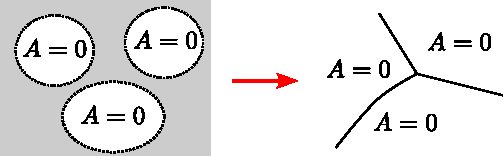
\includegraphics{flatgaugefield.pdf}
  \caption{flatな背景ゲージ場の配位と対称性欠陥の関係。右のようにいろんな点のまわりの球体の領域でゲージ変換を行って$A=0$となるようにする。領域の境目のみで$A\ne 0$になるが、これが対称性欠陥になる。}
  \label{fig:flatgaugefield}
\end{figure}

図\ref{fig:flatgaugefield}を見てもらっても分かるように、この操作を行うと一般的に対称性欠陥が枝分かれしている\kyou{ジャンクション}ができます。ゲージ変換によってジャンクションも連続的に動かすことができるので、このジャンクションもトポロジカルです。このジャンクションで繋がれるトポロジカル欠陥は何でもよいわけではなく、flatであることからジャンクションまわりのWilsonループが1になるので、それぞれの欠陥に割り振られる群の元は
\begin{align}
  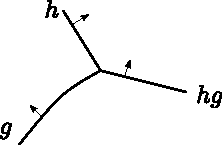
\includegraphics{junction.pdf}
\end{align}
という関係になります。

図\ref{fig:flatgaugefield}では2次元的に書いているので余次元2のジャンクションだけですが、高次元ではこのようなジャンクションがさらに集まったジャンクションもできます。3次元空間の中で泡が集まっているようなものを思い浮かべてください。

まとめると
\begin{emphasize}
  flatなゲージ場の配位は、様々な次元のトポロジカルなジャンクションを含む対称性欠陥の配位で表される。
\end{emphasize}

一般のこのような対称性欠陥の配位の元での分配関数は理論の詳細によります。しかし、対称性のみから導かれるWard-Takahashi恒等式から分かる部分もあります。

\subsection{Ising模型のspin flipの例}\label{sec:egspinflip}
前項までは、連続的な場の理論の描像で対称性がトポロジカル欠陥で表されることを見てきました。連続的な場合には正則化など場の理論特有の微妙な問題もあって、数学的に厳密な取り扱いが難しいです。この項では、格子上でのIsing模型のspin flipの対称性を例にとって、対称性とトポロジカル欠陥を考えてみます。この場合には、経路積分が有限和になりますから、数学的に厳密な取り扱いが可能となります。

まず、Ising模型を定義します。$d$次元の立方格子を考えます。周期境界条件を課して有限個のサイトがあるような場合を考えます。サイトのラベルを$i,j,\dots$とします。各サイト$i$に自由度$a_i=0,1$を置きます。そして$K$を正の実数として、分配関数をすべての$a_i=0,1$の足し上げ
\begin{align}
  Z:=\sum_{\{a\}}e^{-S(a)},\quad
  S(a):=K \sum_{\link{ij}:\text{すべてのリンク}}(-1)^{a_i+a_j}
  \label{ddimIsing}
\end{align}
で定義します。ここでサイト$i,j$をつなぐリンクを$\link{ij}$で表しました。これは有限和ですから、数学的に厳密な取り扱いができます。\footnote{ここで数学的に厳密に取り扱いを説明するという意味ではありません。}

このIsing模型にはspin flipの対称性
\begin{align}
  a_i \to a_i+1 \mod{2}
\end{align}
があります。この対称性を表すトポロジカル欠陥がどのようなものかを考えてみましょう。そのために領域(サイトの集合)$D$をとり、変換
\begin{align}
  a'_i=
  \begin{cases}
    a_i+1,& i\in D\\
    a_i,& i \notin D
  \end{cases}
  \label{gaugespinflip}
\end{align}
を考えます。ここで、\eqref{ddimIsing}の分配関数は
\begin{align}
  Z=\sum_{\{a\}}e^{-S(a)}=\sum_{\{a'\}}e^{-S(a')}=\sum_{\{a\}}e^{-S_{D}(a)}
\end{align}
と変形できます。最初は和を取っている変数の文字を変えただけです。次は\eqref{gaugespinflip}を代入し、明らかに成り立つ性質$\sum_{\{a'\}}=\sum_{\{a\}}$を用いました。また、$S_{D}(a):=S(a')$を定義しました。

$S_{D}(a)$と$S(a)$の違いを見てみましょう。リンク$\link{ij}$に関して、$i,j\notin D$の場合には変換しないので変化なし、$i,j\in D$の場合にも両方のスピンが反転するので、相互作用は変化しません。変化するのは片方が$D$に入っていて、もう片方は$D$に入っていない場合、つまりリンクが$D$の境界にある場合です。このようなリンクは、分配関数への寄与が
\begin{align}
  \exp\left(-K(-1)^{a_i+a_j}\right)
\end{align}
と反強磁性の相互作用になります。したがって$M=\del D$の部分でのみ相互作用が反強磁性になっていて、他の部分と異なっています。したがって、これは余次元1の欠陥になります。また、いろんな領域をとって\eqref{gaugespinflip}の変換をすることによって、分配関数の値を変えずに連続的に\footnote{格子理論で「連続的」は奇妙な感じがしますが、ここでは、境界付近にあるサイト一つだけまたぐ変形を繰り返してできる変形を「連続的な変形」と呼んでいます。}欠陥を動かすことができるので、この欠陥はトポロジカルです。つまり、この欠陥が対称性を表すトポロジカル欠陥である「対称性欠陥」です。

このspin flipのトポロジカル欠陥とゲージ場の配位の関係についても見ておきましょう。先程出てきた$S_{D}$は次のように書くことができます。
\begin{align}
  S_{D}(a):=-K\sum_{\link{ij}}(-1)^{a_i+a_j+b_{ij}},\quad
  b_{ij}=\begin{cases}
    0, & \link{ij}\notin M\\
    1, & \link{ij} \in M
  \end{cases}.
\end{align}
この$b_{ij}$は、リンクに群$\Zb_2$の元$0,1$が配置されているので、格子理論における$\Zb_2$背景ゲージ場と思うことができます。
格子ゲージ理論については、後ほど詳しく説明します。このゲージ場の配位$b_{ij}$は次のようにflatという性質を満たします。格子においてサイトを頂点とする最小の正方形をプラケット(plaquette)と呼ぶことにします。任意のプラケットをとってきて、それを囲む4つのリンクを$\link{ij},\link{jk},\link{kl},\link{li}$とします。このとき上の$b$は
\begin{align}
  b_{ij}+b_{jk}+b_{kl}+b_{li}=0 \mod{2}
\end{align}
を満たします。このようなゲージの配位はflatな配位といいます。

逆にflatなゲージ場の配位が与えられたとします。すると$b_{ij}=1$となるようなリンクを横切るように欠陥を繋いでいくことで、対称性欠陥の配位と思うことができます。対称性欠陥が端がなく、ちゃんとつながっていることは次のように保証されます。flatなので、すべてのプラケットに関して$b_{ij}=1$のリンクは偶数個あります。ですから、あるプラケットに入ってきた欠陥は、必ず出ていくことができます。

\section{対称性欠陥のまとめ}
これまでいろんな面から対称性の見方③余次元1のトポロジカル欠陥で群構造を持つもの、というのを見てきました。その声質をまとめておきます。

普通の対称性は次のようなものです。群$G$を考えます。$\forall g\in G$と時空の中の余次元1の向きのついた面$M$に対して、トポロジカル欠陥$U_{g}(M)$があって次のような性質を満たします。
\begin{itemize}
  \item 群構造
  \begin{enumerate}
    \item フュージョン(fusion)は群の積。
    \begin{align}
      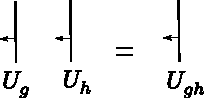
\includegraphics{groupmul.pdf}
    \end{align}
    \item 群の単位元には、自明な欠陥が対応。
    \begin{align}
      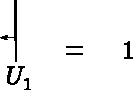
\includegraphics{groupidentity.pdf}
    \end{align}
    \item 逆元に対応するのは、向きを裏返したものである。
    \begin{align}
      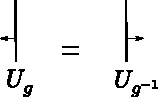
\includegraphics{groupinverse.pdf}
    \end{align}
  \end{enumerate}
  \item 局所演算子への作用
  \begin{align}
    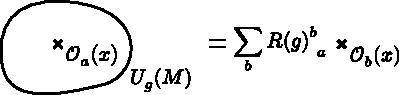
\includegraphics{EgWTid2.pdf}
  \end{align}
\end{itemize}

\section{一般化対称性}
これまで、普通の対称性がある種のトポロジカル欠陥という見方ができることが分かりました。逆に一般のトポロジカル欠陥欠陥は必ずしも対称性を表すものではありません。ここでのアイデアは、これを逆手にとって対称性の一般化を行うことです。
\begin{emphasize}
  一般のトポロジカル欠陥を\kyou{「一般化対称性」}と呼ぶ。
\end{emphasize}

まず、対称性はトポロジカル欠陥のうちで特殊なものでしたから、トポロジカル欠陥のことを一般化対称性と呼ぶのは妥当なことだと思います。大事なことはこの一般化対称性が普通の対称性と同じように場の理論の解析に使えるかということです。まず、トポロジカルという性質だけからWard-Takahashi恒等式に当たる恒等式を考えることができます。また導入の章で説明した例ですと、Hamiltonianと交換するというのはトポロジカルということです。この性質があると、普通の対称性でなかったとしても、ある場面では対称性と同様の使い方ができるということは、導入の章で説明したとおりです。ただし、一般化対称性をどのように使うかということに関しては、まだまだ研究の余地があり、現在も発展中です。

普通の対称性とは異なる一般化対称性には、ざっくり2つの方向性があります(もちろん両方の意味で一般化することも考えます)。
\begin{itemize}
  \item 普通の対称性は余次元1でしたが、これを余次元$p+1,\ p>0$にしたものは$p$形式対称性とか高次形式対称性と呼ばれます。
  \item 群構造が無いトポロジカル欠陥は「非可逆対称性」と呼ばれます。
\end{itemize}

非可逆対称性の名前の由来について、もう少しだけ説明します。まず、2つのトポロジカル欠陥を並べて置いたものはまたトポロジカル欠陥とみなすことができます。このような操作で新しいトポロジカル欠陥を作ることを\kyou{「フュージョン」}(fusion)といいます。これは対称性欠陥のまとめのところでも出てきました。普通の対称性の場合にはフュージョンは群の掛け算になります。また、自明なトポロジカル欠陥(何も置かない)ものは必ず存在します。自明なトポロジカル欠陥は任意のトポロジカル欠陥とフュージョンしても変化させないので、単位元の役割を果たします。つまり、群構造のうちで満たさない可能性があるのは逆元の存在です。考えているトポロジカル欠陥$A$に対して、フュージョンによって$A$を消すようなトポロジカル欠陥が存在しない場合に$A$や$A$を含むようなトポロジカル欠陥の集合を非可逆対称性と呼びます。

空間方向にのみ伸びているトポロジカル欠陥はHilbert空間に作用する演算子で、Hamiltonianと交換するものと思うことができます。このトポロジカル欠陥が非可逆対称性であることは、必ずしも\kyou{このHamiltonianと交換する演算子が逆演算子を持たないということではない}ということに注意してください。トポロジカル欠陥が非可逆というのは逆のトポロジカル欠陥が無いということです。演算子に逆があったとしても、それが非局所的で欠陥ですらないようなものの場合には、トポロジカル欠陥は非可逆といいます。

\chapter{2次元Ising模型}

この章では、2次元Ising模型を題材にして次の2つのことを説明したいと思います。
\begin{itemize}
  \item 2次元Ising模型のspin flipの$\Zb_2$対称性をゲージ化することについて説明します。離散対称性のゲージ化とは何か、そして有限アーベル群をゲージ化したときに必ず現れる大域的対称性「双対対称性」とその性質について説明します。
  \item 非可逆対称性の例とてKramers-Wannier双対性を説明します。
\end{itemize}

\section{2次元Ising模型と\texorpdfstring{\Ztwo}{Z2}ゲージ化}
\subsection{2次元Ising模型}
まず、Ising模型の作用を書きます。これは前章で導入したものと同じものです。2次元正方格子を周期境界条件で考えます。
各サイトに自由度$a_i=0,1$を置きます。$K$を正の定数として分配関数は
\begin{align}
  \ZIsing(K) =\sum_{\{a\}} \exp (K\sum_{\link{ij}}(-1)^{a_i+a_j})\label{ZIsing}
\end{align}
とします。

この系にはspin flipの大域的対称性があります。
\begin{align}
  a_i\to a_i+1 \mod{2}.
\end{align}

\subsection{ゲージ化}\label{sec:gauging}
Spin flipの$\Zb_2$の対称性をゲージ化するすることを考えます。

ゲージ場は各リンク$\link{ij}$に$\Zb_2$に値を持つ自由度$b_{ij}=0,1$として導入します。前節では背景ゲージ場として同じものが現れましたが、ここでは動的な自由度として導入します。

ゲージ変換はパラメータを各サイトに割り振られた$\Zb_2$の元$\lambda_i=0,1$として、
\begin{align}
  b'_{ij}&=b_{ij}+\lambda_i+\lambda_j,\notag\\
  a'_{i}&=a_{i}+\lambda_i
\end{align}
とします。

\eqref{ZIsing}を変形して、トポロジカルにゲージ化された理論の分配関数を$V$をサイトの数として
\begin{align}
  \Zgauged(K) = \frac{1}{2^V}\sum_{\{a\},\{b\}} \exp(K\sum_{\link{ij}} (-1)^{a_i+a_j+b_{ij}})\prod_{\text{すべてのプラケット}\plaq{ijkl}}\deltamod{b_{ij}+b_{jk}+b_{kl}+b_{li},0}
  \label{gaugedIsing}
\end{align}
と定義します。この分配関数について少し説明します。

まず、先頭についている$\frac{1}{2^V}$の分母$2^V$は、「ゲージ体積」です。ゲージ対称性でつながるような配位は物理的に同じ配位とみなすので、分配関数はその冗長性で割っておく必要があります。

最後についている$\deltamod{}$のところについて説明します。まず、この記号は$b$を整数として
\begin{align}
  \deltamod{b,0}=
  \begin{cases}
    1, & b=0\mod{2}\\
    0, & b=1\mod{2}
  \end{cases}
  \label{deltamod2}
\end{align}
と定義します。つまり全てのプラケットについて4辺の$b$の和が偶数の配位、つまりflatな配位のみ足し合わせるということにしています。このような拘束条件をつけたゲージ化を「トポロジカルなゲージ化」と呼ぶことにします。格子の場合には、離散対称性をゲージ化する場合に必ずこのようにしなければならないということではありません。ゲージ場の作用として別のものを選んで、flatに限らないゲージ場の配位をすべて足し合わせるようなゲージ化も可能です。ここでは後のためにトポロジカルなゲージ化を考えようということです。この講義に出てくる離散対称性のゲージ化は8割くらいがこのトポロジカルなゲージ化です。この講義でも後でトポロジカルではないゲージ理論を考えます。論文に出てくる離散対称性のゲージ理論は9割以上がトポロジカルなゲージ化です。

トポロジカルなゲージ化は非常に特殊なことをやっているように見えますが、実はWilsonのプラケット作用で弱結合極限を考えたものとみなすことができます。
\begin{align}
  \deltamod{b,0}=\lim_{g\to 0} \exp(\frac{1}{g^2}((-1)^{b}-1))
\end{align}
という恒等式が成り立ちます。この式の右辺のexpの中で$b$としてプラケットのリンク変数を全部足したものを代入したものがWilsonのプラケット作用のプラケットの重みでしたから、式\eqref{gaugedIsing}の左辺の$\deltamod{}$の積の項はWilsonのプラケット作用で弱結合極限をとったものとみなすことができます。

\subsection{ゲージ固定}
前章でflatな背景ゲージ場の配位は対称性欠陥の配位と同等であることを見ました。今、トポロジカルなゲージ化では、それぞれのゲージ場の配位はflatなので、対称性欠陥の配位と思うことができます。つまり、ゲージ化とは、すべての対称性欠陥の配位について足し合わせることです。これを\eqref{gaugedIsing}の分配関数で実際に見てみたいと思います。

\eqref{gaugedIsing}では、ゲージ変換でつながっている、物理的には同等な配位を何回も足しています。これを次のようにしてゲージ変換でつながっている対称性は1回だけ足すように変形します。こうすると、ゲージ場に関する和の項の数は非常に少なくなりますが、代わりに欠陥がある特別なリンクが出てきて、格子の並進対称性が明白では無くなります。\footnote{もちろん理論として格子の並進対称性は存在します。並進変換するとゲージ固定条件がこわれますが、ゲージ変換をすることでゲージ固定条件を再び満たすようにできます。これらの変換を組み合わせたものがゲージ固定した後の並進対称性です。}

\begin{figure}
  \centering
  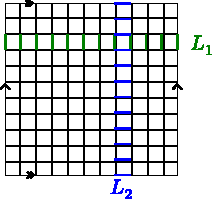
\includegraphics{gaugefix.pdf}
  \caption{ゲージ固定に用いるリンクの列。}
  \label{fig:gaugefix}
\end{figure}


\newcommand{\torusoo}{
  \ 
  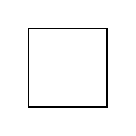
\begin{tikzpicture}[baseline=0.4cm]
    \draw (0,0) rectangle (1,1);   
  \end{tikzpicture}
  \ 
}

\newcommand{\torusio}{
  \ 
  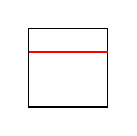
\begin{tikzpicture}[baseline=0.4cm]
    \draw (0,0) rectangle (1,1);   
    \draw[thick,red] (0,0.7)--(1,0.7); 
  \end{tikzpicture}
  \ 
}

\newcommand{\torusoi}{
  \ 
  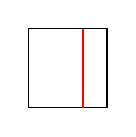
\begin{tikzpicture}[baseline=0.4cm]
    \draw (0,0) rectangle (1,1);   
    \draw[thick,red] (0.7,0)--(0.7,1); 
  \end{tikzpicture}
  \ 
}

\newcommand{\torusii}{
  \ 
  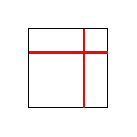
\begin{tikzpicture}[baseline=0.4cm]
    \draw (0,0) rectangle (1,1);   
    \draw[thick,red] (0,0.7)--(1,0.7); 
    \draw[thick,red] (0.7,0)--(0.7,1); 
  \end{tikzpicture}
  \ 
}


まず、図\ref{fig:gaugefix}のように縦方向のリンクの横方向の列$L_1$と横方向のリンクの縦方向の列$L_2$を選びます。任意のflatな$b$の配位において、ゲージ変換で$L_1,L_2$以外のリンクの$b$をすべて$0$にできます。
\begin{align}
  b_{\ell}=0,\ \ell \ne L_1, L_2.
\end{align}
こういうふうにゲージ固定した上で、$L_1$の中にあるリンクについて考えましょう。flatであることと、接している横方向のリンクの$b$が、$L_2$と交わるところ以外で$0$であることから、となり同士の$b$の値は等しくなります。ですから$L_1$に属するすべてのリンクの$b$の値は等しくなります。同様の考察を$L_2$に関しても行うことができます。まとめると、ゲージ固定した後のゲージ場の配位は次の4種類になります。
\begin{align}
  \ell_1\in L_1,\ \ell_2 \in L_2,\quad (b_{\ell_1},b_{\ell_2})=(0,0),(1,0),(0,1),(1,1)
\end{align}
この4つの配位はゲージ不変であるWilsonループの値が異なりますから、ゲージ変換では繋がらない配位です。また、$b_{\ell_1}=1$の場合には$L_1$のところに\ref{sec:egspinflip}項で考えたspin flipの欠陥が入っている配位です。$b_{\ell_1}=0$の場合には$L_1$には欠陥は入っていないと言うこともできますし、自明な欠陥が入っていると言っても良いです。$L_2$の方も同様で、自明な欠陥が入っている場合と、spin flipの欠陥が入っている場合があります。$(b_{\ell_1},b_{\ell_2})=(0,0),(1,0),(0,1),(1,1)$場合の欠陥が入ったIsing模型の分配関数を、それぞれspin flip欠陥を赤線で描いた絵を用いて$\torusoo,
\torusio,\torusoi,\torusii$で表すことにします。

次に全体にかかる定数の規格化を求めるために、このゲージ固定をした後で残っているゲージ対称性について考えましょう。残っているゲージ対称性、つまりゲージ固定条件を変えないゲージ変換のパラメーターは次の2種類だけです。
\begin{align}
  \lambda_i=0\ (\text{すべての}i),\quad \lambda_i=1\ (\text{すべての}i).
\end{align}
言い換えると、ゲージ体積のうち$2$以外は、このゲージ固定から出てくる冗長性と相殺しています。

これらを合わせると、\eqref{gaugedIsing}の分配関数は
\begin{align}
  \Zgauged=\frac{1}{2}\left(
    \torusoo + \torusio + \torusoi + \torusii
  \right)
\end{align}
となります。

\section{双対対称性}\label{sec:dualsymmetry}
この節では、Ising模型を離れて、一般的な2次元の場の理論での有限アーベル群の大域的対称性とそのゲージ化について考えます。

$G$を有限アーベル群、$\Tcal$を2次元の場の理論で大域的$G$対称性があり、$G$はゲージ化可能であるものとします。言い換えると$\Tcal$の$G$対称性には't Hooftアノマリーは無いものとします。$\Tcal$の$G$対称性をゲージ化した理論を$\Tcal/G$と表すことにします。

このとき、次のような命題が成り立ちます。
\begin{proposition}[命題]
  \begin{enumerate}
    \item[(1)] $\Tcal/G$には$\Gh$(Pontryagin 双対)の大域的対称性があります。この$\Gh$対称性にはアノマリーはありません。
    \item[(2)] $\Tcal/G/\Gh \cong \Tcal.$
  \end{enumerate}      
\end{proposition}
Pontryagin双対$\Gh$について説明します。$\Gh$は集合として
\begin{align}
  \Gh=\{G\text{の既約表現}\}/(\text{同値})
\end{align}
です。アーベル群の既約表現ですから、すべて1次元表現です。群の掛け算は表現のテンソル積$\otimes$で定義します。テンソル積はまた1次元表現になるので、既約表現です。単位元は自明な表現、逆元は双対表現になって$\Gh$は群をなします。別の言い方をすると、$\Gh$は$G$対称性のあり得る電荷の集合です。電荷には足し算の概念があって、それで群になります。

この命題について説明していきます。まず、(1)について説明します。前章で説明したとおり、対称性とは余次元1のトポロジカル欠陥で群構造を持つ「対称性欠陥」で表されるのでした。今の場合、\kyou{Wilsonループが対称性欠陥になります。}ゲージ理論においてWilsonループはゲージ群$G$の表現でラベルされる次元1の欠陥です。今は全体の次元が2ですからWilsonループの余次元は1になります。また、今はトポロジカルなゲージ化を考えているので、場の強さは$0$であり、Wilsonループは連続的に変形しても値を変えない、つまりトポロジカルになります。さらに、Wilsonループのフュージョンは表現のテンソル積になります。上で見たように、有限アーベル群の既約表現全体$\Gh$はまたテンソル積でアーベル群になります。こうして、Wilsonループが対称性を表す対称性欠陥であり、対称性の群は$\Gh$ことが分かります。

次に(2)について説明します。簡単のためにトーラスの分配関数を考えます。まず、理論$\Tcal$の分配関数を
\begin{align}
  Z_{\Tcal}=
    \ 
    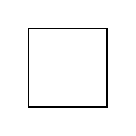
\begin{tikzpicture}[baseline=0.4cm]
      \draw (0,0) rectangle (1,1);   
    \end{tikzpicture}
    \ 
\end{align}
$N:=|G|$として、$\Tcal/G$の分配関数は、すべての対称性欠陥の配位を足し上げることで得られるので
\begin{align}
  Z_{\Tcal/G}=\frac{1}{N}
  \sum_{a,b\in G}
    \ 
    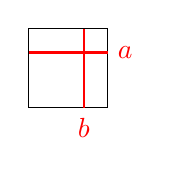
\begin{tikzpicture}[baseline=0.4cm]
      \draw (0,0) rectangle (1,1);   
      \draw[thick,red] (0,0.7)--(1,0.7) node[right]{$a$}; 
      \draw[thick,red] (0.7,0) node[below]{$b$}--(0.7,1); 
    \end{tikzpicture}
    \ 
    =:
    \ 
    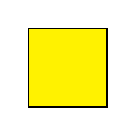
\begin{tikzpicture}[baseline=0.4cm]
      \filldraw[fill=yellow,draw=black] (0,0) rectangle (1,1);
      % \draw[thick,red] (0,0.7)--(1,0.7); 
      % \draw[thick,red] (0.7,0)--(0.7,1); 
    \end{tikzpicture}
    \ 
  \label{T/G}
\end{align}
となります。これを右辺のように黄色い四角で表すことにします。ここから$\Tcal/G/\Gh$の分配関数を考えます。これもWilsonループの配位について足し合わせて
\begin{align}
  Z_{\Tcal/G/\Gh}=\frac{1}{N}\sum_{\ah, \bh \in \Gh}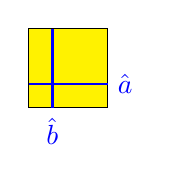
\begin{tikzpicture}[baseline=0.4cm]
    \filldraw[fill=yellow,draw=black] (0,0) rectangle (1,1);
    \draw[thick,blue] (0,0.3)--(1,0.3) node[right]{$\ah$}; 
    \draw[thick,blue] (0.3,0) node[below]{$\bh$}--(0.3,1); 
  \end{tikzpicture}
\end{align}
ここで、$\Gh$対称性の対称性欠陥であるWilsonループを青い線で表しました。これに\eqref{T/G}を代入して
\begin{align}
  Z_{\Tcal/G/\Gh}=\frac{1}{N^2}\sum_{a,b\in G}\sum_{\ah, \bh \in \Gh}
  \ 
  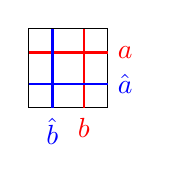
\begin{tikzpicture}[baseline=0.4cm]
    \draw (0,0) rectangle (1,1);   
    \draw[thick,red] (0,0.7)--(1,0.7) node[right]{$a$}; 
    \draw[thick,red] (0.7,0) node[below]{$b$}--(0.7,1); 
    \draw[thick,blue] (0,0.3)--(1,0.3) node[right]{$\ah$}; 
    \draw[thick,blue] (0.3,0) node[below]{$\bh$}--(0.3,1); 
  \end{tikzpicture}
  \ 
  \label{T/G/Gh}
\end{align}
右辺の和の中について考えてみます。これは理論$\Tcal$の中で赤線で表される対称性欠陥、言い換えると背景ゲージ場の下での分配関数に、青線で表されるWilsonループをかけたものです。$\ah$表現での$G$の要素$a$の指標(表現行列のトレース。1次元表現なので$1\times 1$の行列そのもの)を$\chi_{\ah}(a)$とすると
\begin{align}
  \ 
  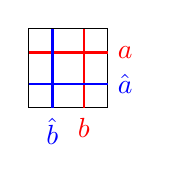
\begin{tikzpicture}[baseline=0.4cm]
    \draw (0,0) rectangle (1,1);   
    \draw[thick,red] (0,0.7)--(1,0.7) node[right]{$a$}; 
    \draw[thick,red] (0.7,0) node[below]{$b$}--(0.7,1); 
    \draw[thick,blue] (0,0.3)--(1,0.3) node[right]{$\ah$}; 
    \draw[thick,blue] (0.3,0) node[below]{$\bh$}--(0.3,1); 
  \end{tikzpicture}
  \ 
  = \chi_{\bh}(a)\chi_{\ah}(b)
  \ 
  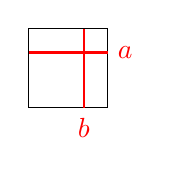
\begin{tikzpicture}[baseline=0.4cm]
    \draw (0,0) rectangle (1,1);   
    \draw[thick,red] (0,0.7)--(1,0.7) node[right]{$a$}; 
    \draw[thick,red] (0.7,0) node[below]{$b$}--(0.7,1);
  \end{tikzpicture}
  \ 
\end{align}
となります。ところで指標は
\begin{align}
  \sum_{\ah \in G}\chi_{\ah}(a)=N\delta_{a,0}
\end{align}
という関係式を満たします。これらを用いると\eqref{T/G/Gh}は
\begin{align}
  Z_{\Tcal/G/\Gh}
  =\frac{1}{N^2}\sum_{a,b\in G}\sum_{\ah, \bh \in \Gh}
  \chi_{\bh}(a)\chi_{\ah}(b)
  \ 
  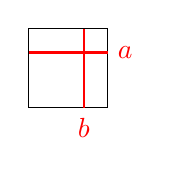
\begin{tikzpicture}[baseline=0.4cm]
    \draw (0,0) rectangle (1,1);   
    \draw[thick,red] (0,0.7)--(1,0.7) node[right]{$a$}; 
    \draw[thick,red] (0.7,0) node[below]{$b$}--(0.7,1); 
  \end{tikzpicture}
  \ 
  =\sum_{a,b\in G}\delta_{a,0}\delta_{b,0}
  \ 
  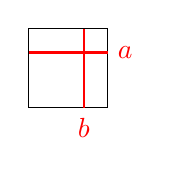
\begin{tikzpicture}[baseline=0.4cm]
    \draw (0,0) rectangle (1,1);   
    \draw[thick,red] (0,0.7)--(1,0.7) node[right]{$a$}; 
    \draw[thick,red] (0.7,0) node[below]{$b$}--(0.7,1); 
  \end{tikzpicture}
  \ 
  =
  \ 
  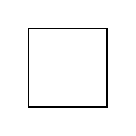
\begin{tikzpicture}[baseline=0.4cm]
    \draw (0,0) rectangle (1,1);   
  \end{tikzpicture}
  \ 
  =Z_{\Tcal}
\end{align}
となります。

先ほどはトーラスの分配関数を考えましたが、一般の閉じたRiemann面を考えるときには計量に関する相殺項に関して少し注意が必要です。まず、特に計量に関する相殺項を入れなかったとすると、その分配関数は
\begin{align}
  Z_{\Tcal/G/\Gh}=\frac{1}{N^{\chi}}Z_{\Tcal}
\end{align}
となります。ここで$\chi$はRiemann面Euler数で、種数$g$や面、辺、頂点の数(それぞれ$F,E,V$)と
\begin{align}
  \chi=2-2g=F-E+V
\end{align}
の関係にあります。トーラスの場合には、たまたま$\chi=0$なので、先ほどは考える必要がありませんでした。2回やって元にもどるという関係にしたいときには、次のような局所相殺項を入れてゲージ化を定義する必要があります。
\begin{align}
  Z_{\Tcal/G,\text{new}}=\sqrt{N}^{\chi}Z_{\Tcal/G, \text{いままでの}}.\label{Eulercounterterm}
\end{align}
こうすると、一般の閉じたRiemann面で
\begin{align}
  Z_{\Tcal/G/\Gh,\text{new}}=Z_{\Tcal,\text{new}}
\end{align}
となります。このEuler相殺項については、Kramers-Wannier双対性を表す非可逆なトポロジカル欠陥を考えるときにも必要になります。この講義では、今後ゲージ化の際には、この相殺項を入れたものを考えることにします。

この節では、アーベル群によるゲージ化のみを考えました。では、(有限の)非アーベル群によるゲージ化を考えるとどうなるでしょうか。トポロジカルなゲージ化を考えるので、場の強さが$0$なのは変わりません。したがってWilsonループが余次元1のトポロジカル欠陥になるのも同じです。フュージョンは表現のテンソル積になるのも同じです。違いは非アーベル群の場合には、次元が2以上の既約表現があり、テンソル積の意味で逆が無い場合があるということです。つまり、有限非アーベル群をゲージ化した際の双対対称性(よく$\mathrm{Rep}(G)$と書かれます)は、トポロジカル欠陥で群構造がない「非可逆対称性」になっています。おそらくこれが非可逆対称性の一番簡単な例です。この例も含め2次元の非可逆対称性については\cite{Bhardwaj:2017xup}に詳しく説明されています。この講義では$\mathrm{Rep}(G)$はこれ以上説明しません。もう一つの代表的な非可逆対称性の例で高次元にも類似物があるKramers-Wannier双対性について詳しく説明します。

\section{Kramers-Wannier 双対性}
この節では、2次元Ising模型のKramers-Wanner双対性を紹介します。Kramers-Wanner双対性はよく統計力学の教科書でも紹介されていますが、ここでは後のためにより精密な双対性について述べます。後に、このKramers-Wanner双対性に対応する非可逆対称性について述べます。

また、Kramers-Wannier双対性とIsing模型の相構造について述べます。

\subsection{Kramers-Wannier双対性と、その証明}\label{sec:KWproof}

\begin{proposition}[Kramers-Wanner双対性]
次の恒等式が厳密に成り立ちます。
\begin{align}
  \frac{1}{(\sinh 2K)^{V/2}} \Zgauged(K)
  =
  \frac{1}{(\sinh 2\Kt)^{V/2}} \ZIsing(\Kt).
  \label{KWduality}
\end{align}
ここで$K$と$\Kt$は
\begin{align}
  \sinh 2K \sinh 2\Kt =1
  \label{dualrelation0}
\end{align}
の関係で結びついています。
\end{proposition}
分配関数の前についている$\sinh$が入った因子は計量のみによく局所的な項として作用に組み込むことができますから、パラメーターが$K$のゲージ化したIsing模型とパラメーターが$\Kt$のIsing模型は同じ理論であるというのが、この命題です。

この命題を証明します。

まず、\eqref{gaugedIsing}を補助的な変数を用いて書き換えます。\eqref{deltamod2}は
\begin{align}
  \deltamod{b,0}=\frac{1}{2}\sum_{c=0,1}e^{\pi i cb}
\end{align}
という恒等式を満たすことに注目します。すると各プラケット$p$に$c_{p}=0,1$の補助的な自由度を置いて\eqref{gaugedIsing}は
\begin{align}
  \Zgauged(K) = \frac{1}{2^{2V}}\sum_{\{a\},\{b\},\{c\}} \exp(K\sum_{\link{ij}} (-1)^{a_i+a_j+b_{ij}}+\pi i\sum_{\substack{\text{プラケット}\\ p=\plaq{ijkl}}} c_{p}(b_{ij}+b_{jk}+b_{kl}+b_{li}))
  \label{gaugedIsing2}
\end{align}
と書くことができます。ここで、プラケットの数は頂点の数と同じであることを用いました。

\eqref{gaugedIsing2}で、ゲージ対称性を用いて、すべてのサイト$i$で$a_i=0$となるようにゲージ固定します。この固定によって$2^V$個のすべてのゲージ体積を相殺します。その後に$\{b\}$の和を評価します。各リンク$\ell$に対して2つのプラケットが接していることに注目して
\begin{align}
  \Zgauged(K)&=\frac{1}{2^{V}}\sum_{\{c\}}\prod_{\text{リンク}\ell}Z_{\ell},\\
  Z_{\ell}&=\sum_{b=0,1}\exp(K(-1)^{b}+\pi i b(c_p+c_q))\label{KWaux1}\\
  &\qquad (p,q \text{は$\ell$に接している2つのプラケット})\notag
\end{align}
と書くことができます。$Z_{\ell}$の表式では、和をとっているダミーの変数は$b_{\ell}$だったものですが、ダミーの変数ですから単に$b$と書いています。

$c:=c_{p}+c_{q} \mod 2$と略記して、$Z_{\ell}$を変形していきます。
\begin{align}
  Z_{\ell}&=e^{K}+(-1)^{c}e^{-K}\notag\\
  &=\begin{cases}
    2\cosh K & (c=0)\\
    2\sinh K & (c=1)
  \end{cases}\notag \\
  &= 2 \cosh K (\tanh K)^{c} \label{Zell0}
\end{align}
という形に書けます。ここで
\begin{align}
  \tanh K =: e^{-2\Kt}\label{defKt}
\end{align}
の式で$\Kt$を定義します。すると
\begin{align}
  \sinh 2K \sinh 2\Kt =1,\label{dualrelation}\\
  Z_{\ell}=\sqrt{2\sinh 2K} e^{\Kt(-1)^{c}}\label{Zell}
\end{align}
という式が成り立ちます。これらを順に導出していきます。

まず、\eqref{dualrelation}を導出します。\eqref{defKt}の両辺の逆数をとったものから、\eqref{defKt}を引き算します。すると
\begin{align}
  (\text{右辺})&=e^{2\Kt}-e^{-2\Kt}=2\sinh 2\Kt,\\
  (\text{左辺})&=\coth K -\tanh K
  =\frac{\cosh^2 K -\sinh^2 K}{\cosh K \sinh K}
  =\frac{2}{\sinh 2K}
\end{align}
と計算できるので、\eqref{dualrelation}が成り立つことが分かります。

次に、\eqref{Zell}を導出します。\eqref{Zell0}に\eqref{defKt}を代入し、$(-1)^c=1-2c$に注目して変形します。
\begin{align}
  Z_{\ell}=&
  2\cosh K e^{\Kt(-2c)}=
  2\cosh K e^{-\Kt}e^{\Kt(-1)^c}\notag\\&=
  2\cosh K \sqrt{\tanh K}e^{\Kt(-1)^c}=
  \sqrt{2\sinh 2K}e^{\Kt(-1)^c}
\end{align}
と変形できるので\eqref{Zell}が成り立つことが分かります。

\eqref{Zell}を\eqref{KWaux1}に代入して変形します。元の格子に双対な格子を導入すると$\ell$に双対なリンクは双対格子のサイト$p,q$をつなぐ双対格子のリンク$\link{pq}$になります。これを踏まえて式変形すると
\begin{align}
 \Zgauged(K)&=\frac{1}{2^V}\sum_{\{c\}}\prod_{\link{pq}}\sqrt{2\sinh 2K}e^{\Kt(-1)^{c_p+c_q}}
 =(\sinh 2K)^{V}\sum_{\{c\}}\exp\left(\sum_{\link{pq}}\Kt(-1)^{c_p+c_q}\right)\notag\\
 &=(\sinh 2K)^{V} \ZIsing(\Kt)
\end{align}
という式を得ます。ここで\eqref{dualrelation}を用いると\eqref{KWduality}を得ます。また\eqref{dualrelation0}は、\eqref{dualrelation}です。\qed

このKramers-Wannier双対性の証明を見てみると、次の重要な事実が分かります。\kyou{Kramers-Wannier双対性の左辺のゲージ化したIsing模型の格子と右辺のIsing模型の格子は互いに双対関係にあります。}この事実は、後にKramers-Wannier双対性を表すトポロジカル欠陥を考える際に非常に重要な役割を果たします。また、今回見たように、トーラス上で正方格子で考えた場合には、双対の格子は同型になってしまうので分かりにくいですが、一般の格子でのKramers-Wannier双対性の両辺は格子は互いに双対の(一般に異なる)格子になります。

\subsection{Ising模型の相構造}
このKramers-Wannier双対性を踏まえて、Ising模型の相構造について考えてみます。

統計力学の授業などで、Ising模型には相転移があることを聞いたことがあると思います。$K$が大きいところ(低温)では、spin flipの対称性が自発的に破れた相になっています。場の量子論の見方で言えば、ここでは真空が縮退しています。一方で$K$が小さいところ(高温)では対称性が回復していて、場の理論の見方では真空は唯一です。この間には相転移が少なくとも一回はあります。

Kramers-Wanner双対性を用いると、この相転移点を求めることができます。まず大事なことは\Ising と\gIsing は、熱力学的な量、例えば自由エネルギー密度は同じです。これを$f(K)$と書くことにします。Kramers-Wanner双対性から$f(K)=f(\Kt)$が導かれます。また、相転移点では$f(K)$が非解析的になっています。$K=K_c$で相転移があるとすると、$f(K)=f(\Kt)$ですから、$K=\Kt_c$でも非解析的、つまり相転移があることになります。\kyou{ここから、相転移が一回だけであることを仮定すると、自己双対の値$K_c=\Kt_c$となること、つまり\eqref{dualrelation0}から$\sinh 2K_c=1$、したがって$K_c=\frac12 \log  (1+\sqrt{2})$となることが分かります。}

自己双対の点$K=K_c$では、\eqref{KWduality}の式は
\begin{align}
  \Zgauged(K_c)=\ZIsing(K)
\end{align}
となります。つまり、この点では\Ising と\gIsing は同じ理論ということになります。後に見るように、この性質から、この点では非可逆対称性があります。


\begin{figure}
  \centering
  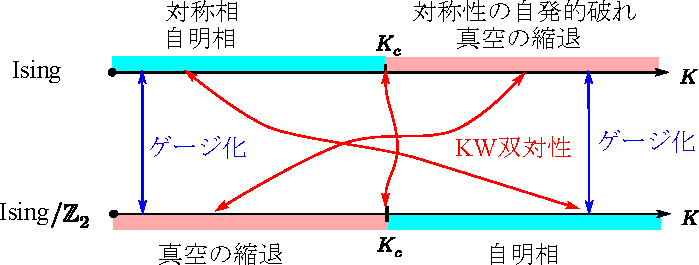
\includegraphics{isingphasestructure.pdf}
  \caption{}
  \label{fig:isingphasestructure}
\end{figure}

もう少し相構造について見てみましょう。図\ref{fig:isingphasestructure}に\Ising と \gIsing の相構造とその関係を示しました。\Ising では$K$が大きいところでは対称性の自発的破れがあり、真空の縮退がありました。Kramers-Wannier双対性から、\gIsing では$K$が小さいところで自発的対称性の破れがあり、真空の縮退があります。\gIsing では、双対$\Zb_2$対称性がありますから、$K$が小さいところでこの対称性が自発的に破れています。一方、\Ising で$K$が小さいところでは対称性が保たれている自明な相になっています。Kramers-Wannier双対性を用いると\gIsing で$K$が大きいところで自明相になっています。

図\ref{fig:isingphasestructure}では、ゲージ化の操作を縦の青い矢印で表しています。例えば$K$が小さいところでは、\Ising は自明相にあり、真空は唯一ですが、これをゲージ化するとゲージ場の自由度を加えることになって、このために真空が縮退します。2つの状態は空間的な円のWilsonループの期待値で区別されます。一方、\Ising で$K$が大きいところでは、真空は二重に縮退しています。これをゲージ化すると、2つの真空のうち、ゲージ不変な方だけが生き残るので、唯一の真空をもつ自明な相になります。

\section{Ising模型の演算子}
ここでは、前節のKramers-Wannier双対性の議論を踏まえたうえで、Ising模型の様々な演算子(欠陥)についてまとめておきます。

まず、その動機について説明します。一つは後にKramers-Wannier双対性で演算子がどのように移り合うかを説明するためです。

もう一つの動機は、Lagrangianに出てくる場の複合演算子として書けない演算子の例を与えることです。\footnote{この講義では、「演算子」と「欠陥」はほぼ同じ意味で用いていますが、主に欠陥の方を用いています。これは、欠陥の方がLagrangianに出てくる場の複合演算子として書けないかもしれないことが強調されると感じたからです。}
一般に場の理論の(局所)演算子には次のようなものがあります。
\begin{enumerate}
  \item Lagrangianに現れる場。
  \item Lagrangianに現れる場の微分やそれらの関数。複合演算子とも呼ばれる。
  \item その他。
\end{enumerate}
1. は場の理論の教科書などで最初に出てきますし、みなさん馴染みがあると思います。2. もカレントやエネルギー運動量テンソルなどをはじめとして、場の理論では重要な演算子です。3. は要するにLagrangianに現れる場の微分や複合演算子として書けない演算子です。まず、1. 2. 3. の違いは記述の違いであって、物理の違いで無いことに注意してください。物理では3. の演算子も重要になる場面は多数あります。ただ、3. の演算子は分かりにくく、教科書等にあまり出てこないため、馴染みが無い方が多いかもしれません。\kyou{Ising模型の演算子は、Lagrangianに現れる場の微分や複合演算子として書けない例を与えます。}


さて、演算子について説明していきます。ここでは、式\eqref{gaugedIsing2}に含まれる自由度で書ける様々な演算子について考えます。特に、次の3種類について考えます。
\begin{itemize}
  \item $c_p$から作るスピン演算子 (spin operator)$\sigma_{p}=(-1)^{c_p}$
  \item $b_{\ell}$から作るWilsonループ (Wilson loop) 演算子$\eta(C)=(-1)^{\sum_{k}b_{\ell_k}}$。ただし、$C$はリンク$\ell_1,\ell_2,\dots$から作られる閉じたループである。
  \item $a_i$から作るスピン演算子。$\mu_{i}\sim (-1)^{a_i}$
\end{itemize}
これらの演算子を作用\eqref{gaugedIsing2}の中だけで考えるなら、特に問題になることはありません。その演算子の相関関数は通常どおり計算できます。これから考えたいのは上の演算子を、$a,b$の和をとってしまって後だったり、$c$の和をとってしまったりした後で考えることです。注意してほしいのは、このように、ある和を先にとってしまったとしても、これらの演算子が無くなるわけではありません。作用に出てくる場の関数として書けなくなるだけです。

これらの演算子について順に見ていきます。

\subsection{スピン演算子}
まず、スピン演算子$\sigma_{p}=(-1)^{c_p}$について説明します。これは、これだけでゲージ不変なので純粋な局所演算子(genuine local operator)です。これは、$a,b$を積分してしまって通常のIsing模型の記述にした後も、そのスピン演算子として、相転移の秩序変数となる重要な演算子です。

一方で、$c$を先に和をとってしまって、\gIsing \eqref{gaugedIsing}の記述にした場合はどうでしょうか。$c$はもはやLagrangianの中に現れる場ではないので、$\sigma_p$ は\kyou{Lagrangianに出てくる場で書けない演算子}になります。では、どう書けるかを考えてみましょう。$\sigma_p=(-1)^{c_p}$を挿入してから$c$について和をとると、\eqref{gaugedIsing}の拘束を表す$\deltamod{}$の因子の中で$\sigma_p$を挿入したプラケット$p$のところだけが、
\begin{align}
  \deltamod{\sum_{\link{ij} \in p}b_{ij}+1,0}
\end{align}
となります。つまり、演算子を挿入したところでは、拘束条件がプラケットでの$b$の和を($0$ではなく)$1$にする、というものになります。

\subsection{対称性欠陥}

次に$b$から作るWilsonループ$\eta$について詳しく見てみます。\ref{sec:dualsymmetry}節で見たように、この$\eta$はトポロジカルで、対称性欠陥になっています。

$\eta$が、スピン演算子$\sigma$を反転するspin flipの演算子になっていることを、詳しく見てみましょう。プラケット$p$に演算子$\sigma_{p}=(-1)^{c_p}$を挿入し、それを囲む経路$C$をとって$\eta(C)$を挿入します。$\eta(C)$はトポロジカルなので、値を変えずに$p$のプラケットまで縮めることができる。作用\eqref{gaugedIsing2}を見ると、この$\eta$の挿入は、和を取っている変数の変換$c_p'=c_p+1$で吸収することができます。このとき$\sigma_{p}=(-1)^{c_p}=-(-1)^{c'_p}$となります。したがって、次のようなWard-Takahashi恒等式が成り立ちます。
\begin{align}
  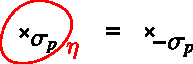
\includegraphics{wtz2.pdf}.
\end{align}
これは、$\eta$がスピン演算子$\sigma$を反転するspin flipの対称性欠陥であることを示しています。

$a,b$を積分してしまった後で$\eta$がどのように表現されるか考えましょう。$\eta(C)$を挿入した後で\ref{sec:KWproof}項と同様に$a,b$の和をとります。すると、$C$に含まれるリンクの相互作用には$(-1)$が余分にかかることになります。つまり
\begin{align}
  \expval{\eta(C)\cdots}
  =\frac{1}{\ZIsing}\sum_{\{c\}}\exp\left(\sum_{\text{すべてのリンク}\link{pq}} \Kt(-1)^{c_p+c_q+\delta_{\expval{pq}}(C)}\right)\cdots
\end{align}
となります。ここで$\delta_{\ell}(C)$はリンク$\ell$が$C$と交わっていれば$1$、そうでなければ$0$という記号です。つまり、$C$と交わっているリンクは、相互作用が反強磁性に置き換わっています。これは\ref{sec:egspinflip}項で見たspin flipの対称性欠陥そのものです。

\subsection{無秩序スピン}
次に無秩序スピンについて詳しく考えてみます。これは、式\eqref{gaugedIsing}の表式でサイト$i$に置かれた演算子$(-1)^{a_i}$です。まず重要なことは$(-1)^{a_i}$そのものはゲージ不変でないので、統計力学での良い演算子ではありません。これが入った相関関数を考えると、いつでも$0$になってしまいます。

\begin{figure}[htbp]
  \centering
  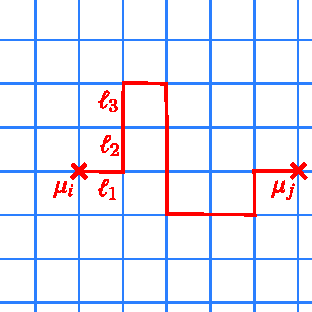
\includegraphics{disorder.pdf}
  \caption{赤い線が$\eta$線演算子で両端の$\mu_i,\mu_j$が無秩序スピン演算子である。この形でゲージ不変になっている。}
  \label{fig:disorder}
\end{figure}

これをゲージ不変にするために$\eta$線演算子($b$ Wilson ライン)をくっつけて
$\mu_i=(-1)^{a_i+b_{\ell_1}+b_{\ell_2}+\dots}$を考えます(図\ref{fig:disorder}参照)。ただし、$\ell_1,\ell_2,\dots$は$i$に端をもつ経路です。この演算子を($(-1)^{c_p}$を秩序演算子としてのスピン演算子と言うのに対応して)無秩序演算子(disorder operator)とか無秩序スピン(disorder spin)と呼びます。\footnote{多くの教科書や論文では、秩序演算子、無秩序演算子の区別は記述によるものです。つまり、Lagrangianに出てくる場で書かれているものが秩序演算子、Lagrangianに出てくる場では書かれていないものが無秩序演算子です。これらは互いに非局所的ですが、どちらが純正な局所演算子かは、気にしていないことが多いです。この講義では、記述にかかわらず、純正局所演算子の方を(秩序)スピン演算子、純正ではなく、トポロジカル欠陥がくっついているものを無秩序スピン演算子と呼ぶことにします。}次のようなことに注意する必要があります。
\begin{itemize}
  \item $\mu_i$は位置$i$だけでなく、くっつくWilsonライン$\eta$の経路によっています。ただし、$\eta$はトポロジカルなので、経路の連続変形にはよっていません。一般に、このような演算子を非純正局所演算子(non-genuine local operator)と呼ぶことがあります。反対の言葉は純正局所演算子(genuine local operator)で、スピン演算子$\sigma_{p}$はその例です\footnote{この``genuine local operator''という用語は文献\cite{Kapustin:2014gua}から使われ始めました。}。
  \item 端のあるWilsonラインは必ず反対側の端があります。したがって$\mu_i$は必ずペアで現れなければなりません。
\end{itemize}

$a,b$の和を取ってしまった後で無秩序スピンがどうなるか見てみましょう。スピン演算子がサイトにあるような格子で考えると、$\mu$はプラケットの中心に配置され、対称性欠陥の端として表されます。別の言い方をすると、プラケット一周してきたときに(周期境界条件ではなく)半周期境界条件を課すという言い方もできます。

\begin{figure}[htbp]
  \centering
  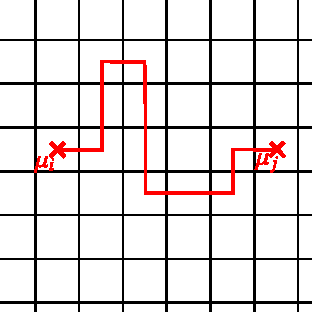
\includegraphics{disorder2.pdf}
  \caption{$a,b$の和をとってしまった後での無秩序演算子の様子。赤で表した経路は対称性欠陥$\eta$を表しています。つまり、赤の線と交わっているリンクは反強磁性になっています。$\mu$演算子は$\eta$の端のプラケットに配置されています。}
  \label{fig:disorder2}
\end{figure}

無秩序スピンの名前の由来は次のようなものです。$\sigma$スピン演算子(秩序スピン演算子)の言葉で秩序相(spin flip対称性が自発的に破れている)にあるときは、$\mu_i$の期待値が$0$になります。正確に言うなら、$\mu$を挿す2点を遠くに離す極限で2点関数が$0$になります。これは次のようにして理解することができます。
秩序相で$K$が大きい極限を考えてみます。このとき、すべてのスピンはそろおうとします。しかし、$\mu$が入っている点のまわりではどこかで反強磁性になっているので、すべてのスピンがそろうことができません。なるべくエネルギーを低くするためには、となりあうスピンが反対の部分(対称性欠陥直上では同じ部分)が最小になるのが、エネルギーが最も低い配位になります。したがって、ある定数$m>0$があって
\begin{align}
  \expval{\mu_{i}\mu_{j}}\sim e^{-m L},\quad (L\text{は$i,j$の間の距離。})
\end{align}
となります。なので$L\to \infty$で2点関数は$0$になります。

一方、無秩序相にあるときは、$\mu$が期待値を持つ、正確には$\mu$を刺す2点を遠くに離す極限で2点関数が$0$でない定数になります。これは次のように理解できます。
無秩序相ではスピンは相関が消えます。ですから、$\mu$演算子が刺さっている点から離れたところではエネルギーに影響はありません。ただし、$\mu$が刺さっていることで、その点の近くでエネルギーが変わりますから、その分$0$でない値が出ます。したがって、$\mu$を挿す2点を遠くに離す極限で2点関数が$0$でない定数になります。

\section{KW欠陥}
これまで準備してきたことを踏まえて、ここでは非可逆対称性の一つの例であるKramers-Wannier (KW)欠陥について紹介します。いろいろな見方があるのですが、ここでは連続理論や高次元への拡張が容易な\kyou{半空間ゲージ化(half-space gauging)}による構成について説明します。

まず、大まかなアイデアについて説明します。一般化対称性とは、何かの方法で作ったトポロジカル欠陥です。最初の方で紹介した対称性の一つの見方①場の変換で作用を不変にするもの、というものがあるとトポロジカル欠陥が作れることを\ref{sec:symmetrydefect}で説明しました。これを絵で表すと
\begin{align}
  \begin{tikzpicture}[baseline=0cm]
    \fill [yellow!80] (0,0) circle [x radius=1.5cm, y radius=1cm, rotate=30];
    \draw[->](1.5,1.5)--(0.5,0.5);
    \node (A) at (1.5,1.5)[above]{変換};
    \node (D) at (0,0){$D$};
  \end{tikzpicture}
  =
  \begin{tikzpicture}[baseline=0cm]
    \draw [red,thick] (0,0) circle [x radius=1.5cm, y radius=1cm, rotate=30];
    \draw[->](1.5,1.5)--(1,1);
    \node (A) at (1.5,1.5)[above]{トポロジカル欠陥};
  \end{tikzpicture}  
  \label{halfspacetransformation}
\end{align}
となります。
これを一般化し、ある領域$D$内で変換だけでなく離散対称性のトポロジカルなゲージ化を含む様々な操作を行うことを考えます。この操作でバルクでは元の理論に戻る場合を考えます。$K=K_c$の場合に$\ZIsing=\Zgauged$でしたから、Ising模型の場合はゲージ化を含む操作で元に戻る、というのが例です。バルクでは元に戻りますから、一般に境界で欠陥ができます。*うまい境界条件*でゲージ化を行うと、この欠陥がトポロジカルになる場合があります。絵で書くと
\begin{align}
  \begin{tikzpicture}[baseline=0cm]
    \fill [blue!10] (0,0) circle [x radius=1.5cm, y radius=1cm, rotate=30];
    \draw[->](1.5,1.5)--(0.5,0.5);
    \node (A) at (1.5,1.5)[above]{\underline{ゲージ化}、変換、補助場の導入、積分、…};
    \node (D) at (0,0){$D$};
  \end{tikzpicture}
  \Rightarrow
  \begin{tikzpicture}[baseline=0cm]
    \draw [green!70!black,thick] (0,0) circle [x radius=1.5cm, y radius=1cm, rotate=30];
    \draw[->](1.5,1.5)--(1,1);
    \node (A) at (1.5,1.5)[above]{トポロジカル欠陥};
  \end{tikzpicture}  
  \label{halfspacegauging}
\end{align}
となります。

ここでいくつかの注意をします。
\begin{itemize}
  \item \eqref{halfspacetransformation}と違って、\eqref{halfspacegauging}は``$=$''の関係でないことに注意してください。これは、あくまで(一般に非可逆な)トポロジカル欠陥を見つける方法であって、Ward-Takahashi恒等式を見つけるには、さらに解析が必要です。
  \item 離散対称性のトポロジカルなゲージ化であったからといって、すぐに境界に現れる欠陥がトポロジカルになるとは言えません。ゲージ化の際のゲージ場の境界条件の取り方は非常に重要です。
\end{itemize}

ここでは、$K=K_c$でのIsing模型を例にとって、この半空間ゲージ化の方法でトポロジカル欠陥を導出します。まず、格子上で領域$D$をどう設定するかについて説明します。これはゲージ場の境界条件と絡んで、重要な部分です。次に半空間ゲージ化の手続きを説明し、バルクがちゃんと元に戻ること、言い換えると現れるトポロジカル欠陥がちゃんと余次元1の欠陥になっていることを説明します。その後に、この欠陥がトポロジカルであることを説明します。

\subsection{領域の取り方}
領域の取り方について詳しく説明します。$\Lambda$を周期境界条件を課した格子とします。この上で$K=K_c$のIsing模型を考えます。分配関数は
\begin{align}
  \ZIsing = \sum_{\{a\}}\exp( K \sum_{\text{リンク}\link{ij}} (-1)^{a_i+a_j})\label{2DIsing}
\end{align}
です。ここで、$i,j$は$\Lambda$のサイトで$a_i$は$\Lambda$のサイトに乗っている自由度です。このようにIsing模型でスピンの自由度がサイトにのっている格子をアクティブ格子(active lattice)と呼ぶことにします。

\begin{figure}
  \centering
  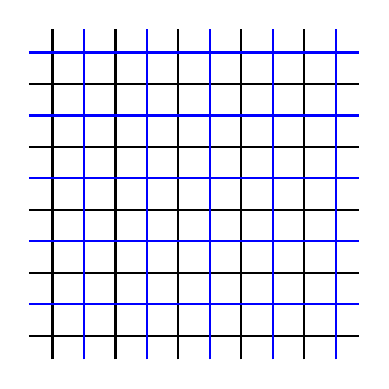
\begin{tikzpicture}
    \draw[step=0.8, thick] (-1.9,-1.9) grid (2.3,2.3);
    \draw[step=0.8, blue, thick, yshift = 0.4cm, xshift = 0.4cm] (-2.3,-2.3) grid (1.9,1.9);            
  \end{tikzpicture}
  \caption{格子$\Lambda$(黒)とその双対格子$\Lambdah$(青)。}\label{fig:lattices}
\end{figure}

さて、$\Lambda$の双対格子である$\Lambdah$(図\ref{fig:lattices}参照)を考えましょう。これは$\Lambda$のプラケットの中心が$\Lambdah$のサイトになるようにとった格子です。今の場合の$\Lambdah$のようにプラケットにスピンの自由度がのっているような格子を非アクティブ格子(innactive lattice)と呼ぶことにします。\ref{sec:KWproof}項で見たとおり、\eqref{2DIsing}を全体でゲージ化すると、$\Lambdah$のサイトにスピンの自由度がのったIsing模型と等価になります。今$K=K_c$を考えているので$K$は変わらないことに注意してください。標語的に言うなら、Kramers-Wannier双対性はアクティブ格子と非アクティブ格子を入れ替えます。

半空間ゲージ化をするときの領域を考えるのに$\Lambdah$の言葉で言うと便利です。
$D$は$\Lambdah$のサイト、リンク、プラケットの集合で、次のような条件を満たすものとします。
\begin{itemize}
  \item プラケット$p\in D$なら、$p$を作る4つのリンクの集合$\del p$は、$\del p \subset D$
  \item リンク$\ell \in D$なら、$\ell$の両端のサイト$i,j$は$i,j\in D$となります。
\end{itemize}
端的に言うなら、$D$は$\Lambdah$の見方で境界が全部含まれるような領域ということになります。

\begin{figure}
  \centering
  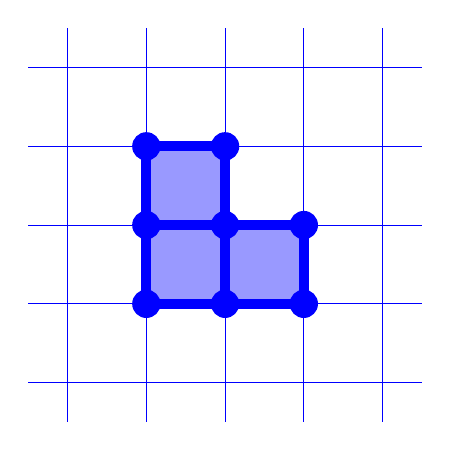
\begin{tikzpicture}
    \draw[step=1, blue] (-1.5,-1.5) grid (3.5,3.5); 
    \foreach \x/\y in {0/0, 0/1, 1/0}{
        \fill[blue!40](\x,\y) rectangle (\x+1,\y+1);
    }
    \foreach \x/\y in {0/0, 0/1, 1/0, 1/1, 0/2, 1/2, 2/0, 2/1}{
        \fill[blue] (\x,\y) circle (1.8mm);
    }
    \foreach \x/\y in {0/0, 0/1, 0/2, 1/0, 1/1}{
    \draw[blue, line width = 1.3mm](\x,\y)--(\x + 1,\y);
    }
    \foreach \x/\y in {0/0, 0/1, 1/0, 1/1, 2/0}{
    \draw[blue, line width = 1.3mm](\x,\y)--(\x,\y+1);
    }
\end{tikzpicture}
\caption{領域$D$の取り方の例。$\Lambdah$の格子を青線で表しています。青丸で表したサイト、太い青線で表したリンク、青く塗っているプラケットが$D$の元です。}
\end{figure}

逆に$\Lambda$の見方では、境界が全部含まれない領域ということになります。後で$D$の中だけでゲージ化するわけですが、このときに境界にある$\Lambda$のリンクにはゲージ場を置かず、また境界にある$\Lambda$のサイトにはゲージ変換を置きません。このような境界条件を\cite{Choi:2021kmx}ではDirichlet境界条件と呼んでいます。後に見るように、この境界条件で半空間ゲージ化をした場合には、境界に残る欠陥がトポロジカルになります。別の境界条件でゲージ化した場合には、トポロジカルになることは保証されません。

\subsection{半空間ゲージ化}\label{sec:halfspacegauging}
ここでは、先に述べた条件を満たす$D$に対して、$D$の中だけでspin flipの対称性をゲージ化する手続きを説明します。しばらくは、言葉の使い方としてサイト、リンク、プラケットなどはすべて$\Lambdah$のものとします。

まず、ゲージ化する前からすべてのプラケット$i$に自由度$a_i=0,1$がのっていて相互作用があるIsing模型を考えていたことを思い出してください。

$D$の要素に関して、次のような変形をします。
\begin{enumerate}
  \item $D$の中の各リンク \tikz[baseline=0.3cm]{\draw[blue, line width = 1.3mm](0,0)--(0,1)} $\ell$ に対して、ゲージ場$b_{\ell}=0,1$を置きます。そしてこのリンクの相互作用を$\exp(K(-1)^{a_i+a_j+b_{\ell}})$とします。ただし、$i,j$はリンクを挟んでいる2つのプラケットです。分配関数の計算では、和$\sum_{b_{\ell}=0,1}$をとります。
  \item $D$の中の各プラケット \tikz[baseline=0.3cm]{\fill[blue!40](0,0) rectangle (1,1);} $i$ に対してゲージ変換を置きます。ゲージ変換のパラメータを$\lambda_i=0,1$とし、このプラケットに置かれている$a_i$とこのプラケットに接しているリンク$\ell$に置かれているゲージ場は
  \begin{align}
    a_i\to a_i+\lambda_i,\quad b_{\ell}\to b_{\ell}+\lambda_i    
  \end{align}
  と変換します。$D$の取り方から、$i$のまわりの4つのリンクはすべて$D$の要素であるので、$b$の自由度が置かれていることに注意してください。

  分配関数を考えるときには、ゲージ体積で割る必要があるので、$D$の要素であるプラケット$i$に対して因子$\frac12$を割り当てます。
  \item $D$の中の各サイト \tikz{\fill[blue] (0,0) circle (1.8mm)} $p$には、ゲージ場$b$がflatでありなさいという拘束条件を置きます。このサイトにつながる4つのリンクのラベルを$1,2,3,4$として
  \begin{align}
    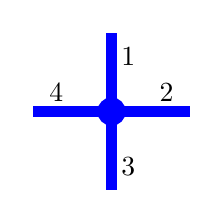
\begin{tikzpicture}[baseline=0]
      \fill[blue] (0,0) circle (1.8mm);
      \foreach \x/\y in {1/0, 0/1, -1/0, 0/-1}{
      \draw[blue, line width = 1.3mm](0,0)--(\x,\y);
      }
      \node (A) at (0,0.7)[right]{$1$};
      \node (B) at (0,-0.7)[right]{$3$};
      \node (C) at (0.7,0)[above]{$2$};
      \node (D) at (-0.7,0)[above]{$4$};
  \end{tikzpicture}\quad \Rightarrow\quad \deltamod{b_1+b_2+b_3+b_4,0}
  =\sum_{c_p=0,1}\frac12 (-1)^{c_p(b_1+b_2+b_3+b_4)}
  \end{align}
  という因子を割り当てます。$D$の中のサイト$p$につながっている4つのリンクは、必ずしもすべてが$D$の元であるとな限らないので、$b$が割り当てられていない場合もあります。このような場合は、$b$が割り当てられていないリンクの$b$は$0$として拘束条件をかします。
  \item \eqref{Eulercounterterm}のあたりで述べたEuler相殺項を考えます。これは多面体に関するEulerの公式を適用すると$D$の要素に対して上で述べた因子の他に
  \begin{align}
    \tikz{\fill[blue] (0,0) circle (1.8mm)}\qquad&\Rightarrow \qquad \sqrt{2}\notag\\
    \tikz[baseline=0.3cm]{\draw[blue, line width = 1.3mm](0,0)--(0,1)} \qquad &\Rightarrow \qquad \frac{1}{\sqrt{2}},\notag\\
    \tikz[baseline=0.3cm]{\fill[blue!40](0,0) rectangle (1,1);} \quad&\Rightarrow \qquad \sqrt{2}
  \end{align}
  という因子を割り当てれば良いことが分かります。
\end{enumerate}

これらをまとめて、$D$で半空間ゲージ化を行った分配関数$Z_{D}$を書いてみます。
\begin{align}
  Z_{D}=&\underrem{\sum_{\{a\}}}{全体にある自由度の和}
  \overrem{\sum_{\{b\}}\sum_{\{c\}}}{D内のみの自由度の和}
  \underrem{\prod_{\text{プラケット }\in D}\sqrt{2}
  \prod_{\text{リンク } \in D}\frac{1}{\sqrt{2}}
  \prod_{\text{サイト} \in D}\sqrt{2}}{Euler相殺項}
  \notag\\
  &\times
  \underrem{\prod_{\text{プラケット }\in D} \frac{1}{2}}{ゲージ体積}
  \underrem{
  \prod_{\text{サイト} \in D}\frac{1}{2}}{拘束を補助場で表したときの$1/2$}
  \notag\\
  &\times
  \prod_{\text{リンク } \notin D}\exp(K(-1)^{a_i+a_j})
  \prod_{\text{リンク } \in D}\exp(K(-1)^{a_i+a_j+b_{ij}})
  \notag\\
  &\times
  \prod_{\text{サイト } p\in D} (-1)^{c_p\sum_{\ell \in p}b_{\ell}}.
  \label{halfspacegauging0}
\end{align}
これから、この分配関数に関して
\begin{itemize}
  \item これが、$D$の境界に局在する余次元$1$の欠陥であること。
  \item この欠陥がトポロジカルであること。
\end{itemize}
の2項目について詳しく見ていきます。

\subsection{境界に局在すること}
まず、境界に局在する欠陥であることを説明します。これには、\ref{sec:KWproof}項でやったのと同様に、$b$について先に和を取ることで理解できます。

まず、ゲージ固定として$D$内のプラケット$i$に関して$a_i=0$というゲージをとります。このゲージ固定により、\eqref{halfspacegauging0}の中のゲージ体積での割り算はすべて相殺します。

次に$b$の和をとることを考えます。$D$内のリンクには2種類あって、リンクの両側のプラケットが両方$D$内にある場合と、片方だけが$D$内にある場合です。前者の場合には、\ref{sec:KWproof}でやったのと全く同じ計算になります。次のように、考えているリンクの変数を$b$、リンクの両端のサイトの自由度を$c_1,c_2$とします。プラケットにある$a$の自由度はすでにゲージ固定で$0$にしていることに注意してください。
\begin{align}
  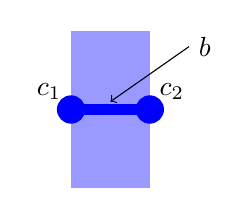
\begin{tikzpicture}
    \coordinate (C1) at (0,0) node [above left] at (C1) {$c_1$};
    \coordinate (C2) at (1,0) node [above right] at (C2) {$c_2$};
    \fill[blue!40](0,0) rectangle (1,1);
    \fill[blue!40](0,-1) rectangle (1,0);
    \fill[blue] (C1) circle (1.8mm);
    \fill[blue] (C2) circle (1.8mm);
    \draw[blue, line width = 1.3mm] (C1)--(C2);
    \coordinate (B) at (1.5,0.8) node [right] at (B){$b$};
    \draw[->] (B)--(0.5,0.1);
\end{tikzpicture}
\end{align}
この$b$を含む部分の和は\ref{sec:KWproof}項と同様に計算して
\begin{align}
  \sum_{b=0,1}e^{K(-1)^{b}}(-1)^{b(c_1+c_2)}
  =\sqrt{2}e^{K(-1)^{c_1+c_2}}
  \label{sumbtemp}
\end{align}
となります。この計算では、今は$K=K_c$の場合を考えているので$\Kt=K,\ \sinh 2K=1$であることに注意してください。\eqref{sumbtemp}の右辺の$\sqrt{2}$は、\eqref{halfspacetransformation}のEuler相殺項のリンクのところとちょうど相殺します。\eqref{sumbtemp}の右辺の残りの部分は、Ising模型のBoltzmannウェイトです。つまり、$D$内のバルクでは$\Lambdah$をアクティブ格子とする、$K=K_c$のIsing模型になっています。

次に、リンクの両側のプラケットのうち、片方のみ$D$の内部にある場合を考えます。$D$の外にあるプラケットにはゲージ対称性は無いので$a$の自由度が残っていることに注意します。次のように自由度の名前をつけます。
\begin{align}
  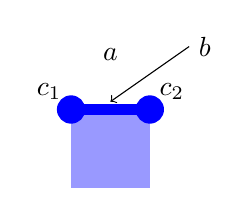
\begin{tikzpicture}
    \coordinate (C1) at (0,0) node [above left] at (C1) {$c_1$};
    \coordinate (C2) at (1,0) node [above right] at (C2) {$c_2$};
    \fill[blue!40](0,-1) rectangle (1,0);
    \fill[blue] (C1) circle (1.8mm);
    \fill[blue] (C2) circle (1.8mm);
    \draw[blue, line width = 1.3mm] (C1)--(C2);
    \coordinate (B) at (1.5,0.8) node [right] at (B){$b$};
    \draw[->] (B)--(0.5,0.1);
    \node (A) at (0.5, 0.7){$a$};
\end{tikzpicture}
\label{boundary}
\end{align}
この部分の$b$の和は、先程と同様に
\begin{align}
  \sum_{b=0,1}e^{K(-1)^{b}}(-1)^{b(c_1+c_2)}
  =\sqrt{2}e^{K(-1)^{c_1+c_2}}(-1)^{ac_1}(-1)^{ac_2}\label{Dboundary}
\end{align}
となります。先ほどと同様に、右辺の$\sqrt{2}$はEuler相殺項のリンクの部分とキャンセルし、次の因子はIsing模型のBoltzmannウェイトになります。それ以外に、$D$の境界上で$(-1)^{ac_1}(-1)^{ac_2}$という因子が残ります。これが本質的に欠陥に与えられるウェイトです。これをまとめて表すために、アクティブサイト(Ising模型の自由度が割り振られているアクティブ格子のサイト)を \tikz{\fill[black] (0.5,0.5) circle (1mm);} で表すことにします。図\ref{fig:KWdefect}を見てください。$D$の外では、$\Lambda$のサイトがアクティブで、その自由度は$a$、$D$の中では、$\Lambdah$のサイトがアクティブで、その自由度を$c$という記号で表してきました。境界では、それらのサイトが隣り合っています。\eqref{Dboundary}の結果は、このように隣り合っているサイトのペアに次のようなウェイトを割り振ればよいということです。
\begin{align}
  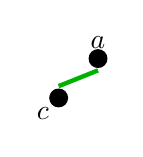
\begin{tikzpicture}
    \foreach \x/\y in {1/0, 0.5/-0.5}{
        \fill[black] (\x,\y) circle (1.2mm);
    }
    \draw[green!70!black, ultra thick](0.5,-0.35)--(1,-0.15);
    \node (C1) at (0.5, -0.5)[below left]{$c$};
    \node (A) at (1, 0)[above]{$a$};
  \end{tikzpicture}
  =(-1)^{ac}
\end{align}

\begin{figure}[htbp]
  \centering
  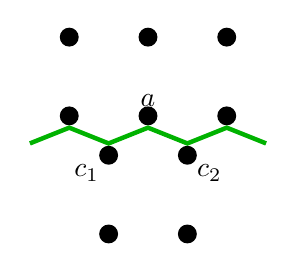
\begin{tikzpicture}
    \foreach \x/\y in {0/0, 0/1, 1/0, 1/1, 2/0, 2/1, 0.5/-0.5, 1.5/-0.5, 0.5/-1.5, 1.5/-1.5}{
        \fill[black] (\x,\y) circle (1.2mm);
    }
    \draw[green!70!black, ultra thick](-0.5,-0.35)--(0,-0.15)--(0.5,-0.35)--(1,-0.15)--(1.5,-0.35)--(2,-0.15)--(2.5,-0.35);
    \node (C1) at (0.5, -0.5)[below left]{$c_1$};
    \node (C2) at (1.5, -0.5)[below right]{$c_2$};
    \node (A) at (1, 0)[above]{$a$};
  \end{tikzpicture}
  \caption{$b$の和を取った後のKW欠陥を説明する図。緑の線を境界として、下が$D$の内側、上が$D$の外側になる。黒い点はIsing模型の自由度が割り当てられたアクティブサイト。アクティブ格子は緑の線を境に互いに双対になっている。}
  \label{fig:KWdefect}
\end{figure}

さて、残り考えないといけないのは、$D$内の各サイトに割り振られた$\sqrt{2}$と$D$内の各プラケットに割り振られた$1/\sqrt{2}$です。境界を気にしなければ、サイトとプラケットは対応させることができるので、このウェイトも境界に押し付けることができます。

最後のところは少し誤魔化しています。本当にこのウェイトがちゃんと境界に押し付けられることを示すには、どのように押し付けるかをちゃんと決める必要があります。これの易しいやり方を私は知りません。実際にちゃんとウェイトを決めることができることが、\cite{Aasen:2016dop}で示されています。

ここまでで、半空間ゲージ化を行うと、その境界に余次元1の欠陥が現れることが分かりました。この欠陥を\kyou{KW欠陥}と呼ぶことにします。

\subsection{トポロジカル性}
次にKW欠陥がトポロジカルであることを示します。

このために$D$を選んで、その要素のサイト、リンク、プラケットをそれぞれ\tikz{\fill[blue] (0,0) circle (1.8mm)}、\tikz[baseline=0.3cm]{\draw[blue, line width = 1.3mm](0,0)--(0,1)}、\tikz[baseline=0.3cm]{\fill[blue!40](0,0) rectangle (1,1);} で表します。これまでやってきたように、$D$で半空間ゲージ化をやった上で、他にも任意の演算子を挿入し、すべての自由度に関して和をとったものに関して成り立つ恒等式(演算子恒等式)を絵で表すことにします。

次の(ア)、(イ)の演算子恒等式が成り立ちます。
\begin{enumerate}
  \item[(ア)] 境界にあるリンク$\ell$とそれを含むプラケット$p$に関して、$p$のゲージ変換で$b_{\ell}=0$にします。このゲージ固定で$p$に割り振られた$1/$ゲージ体積がキャンセルします。またEuler相殺項は$p$と$\ell$で相殺します。結果として、$D$から$p$と$\ell$を除いたもの$D'$で半空間ゲージ化したものと同じになります。
  \begin{align}
    \begin{tikzpicture}[baseline=1cm]
      \foreach \x/\y in {0/0, 0/1, 1/0}{
          \fill[blue!40](\x,\y) rectangle (\x+1,\y+1);
      }
      \foreach \x/\y in {0/0, 0/1, 1/0, 1/1, 0/2, 1/2, 2/0, 2/1}{
          \fill[blue] (\x,\y) circle (1.8mm);
      }
      \foreach \x/\y in {0/0, 0/1, 0/2, 1/0, 1/1}{
      \draw[blue, line width = 1.3mm](\x,\y)--(\x + 1,\y);
      }
      \foreach \x/\y in {0/0, 0/1, 1/0, 1/1, 2/0}{
      \draw[blue, line width = 1.3mm](\x,\y)--(\x,\y+1);
      }
      \draw[<-,thick] (0.5,1.5)--(2,2) node[right] {ゲージを選ぶ};
      \draw[<-,thick] (0.5,2.1)--(2,3) node[right] {$b=0$にする};
      \draw[->,red, line width=2mm](3,2.2)--(3,2.8);
  \end{tikzpicture}
  \quad
  =
  \qquad
  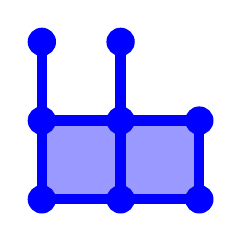
\begin{tikzpicture}[baseline=1cm]
    \foreach \x/\y in {0/0, 1/0}{
        \fill[blue!40](\x,\y) rectangle (\x+1,\y+1);
    }
    \foreach \x/\y in {0/0, 0/1, 1/0, 1/1, 0/2, 1/2, 2/0, 2/1}{
        \fill[blue] (\x,\y) circle (1.8mm);
    }
    \foreach \x/\y in {0/0, 0/1, 1/0, 1/1}{
    \draw[blue, line width = 1.3mm](\x,\y)--(\x + 1,\y);
    }
    \foreach \x/\y in {0/0, 0/1, 1/0, 1/1, 2/0}{
    \draw[blue, line width = 1.3mm](\x,\y)--(\x,\y+1);
    }
  \end{tikzpicture}
  \end{align}
  \item[(イ)] 境界にあるサイト$i$とリンク$\ell$で次を満たすものを考える。
  \begin{enumerate}
    \item $i$につながる4つのリンクで$D$に属するのは$\ell$のみ。
    \item $\ell$の両側にあるプラケットは$D$に属さない。
  \end{enumerate}
  このとき、サイト$i$の拘束条件から$b_{\ell}=0$のみが寄与します。またEuler相殺項は$i$と$\ell$で相殺します。結果として$D$から$i$と$\ell$を除いた$D'$で半空間ゲージ化したものと同じになります。
  \begin{align}
    \begin{tikzpicture}[baseline=1cm]
      \foreach \x/\y in {0/0, 1/0}{
          \fill[blue!40](\x,\y) rectangle (\x+1,\y+1);
      }
      \foreach \x/\y in {0/0, 0/1, 1/0, 1/1, 0/2, 1/2, 2/0, 2/1}{
          \fill[blue] (\x,\y) circle (1.8mm);
      }
      \foreach \x/\y in {0/0, 0/1, 1/0, 1/1}{
      \draw[blue, line width = 1.3mm](\x,\y)--(\x + 1,\y);
      }
      \foreach \x/\y in {0/0, 0/1, 1/0, 1/1, 2/0}{
      \draw[blue, line width = 1.3mm](\x,\y)--(\x,\y+1);
      }
      \draw[<-,thick] (1.1,1.5)--(2,2) node[right] {$b=0$のみ};
      \draw[<-,thick] (1.1,2.1)--(2,3) node[right] {拘束条件};
      \draw[<-,red, line width=2mm](3,2.2)--(3,2.8);
  \end{tikzpicture}
    \quad
    =
    \qquad
    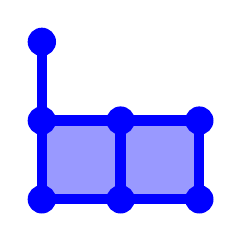
\begin{tikzpicture}[baseline=1cm]
      \foreach \x/\y in {0/0, 1/0}{
          \fill[blue!40](\x,\y) rectangle (\x+1,\y+1);
      }
      \foreach \x/\y in {0/0, 0/1, 1/0, 1/1, 0/2, 2/0, 2/1}{
          \fill[blue] (\x,\y) circle (1.8mm);
      }
      \foreach \x/\y in {0/0, 0/1, 1/0, 1/1}{
      \draw[blue, line width = 1.3mm](\x,\y)--(\x + 1,\y);
      }
      \foreach \x/\y in {0/0, 0/1, 1/0, 2/0}{
      \draw[blue, line width = 1.3mm](\x,\y)--(\x,\y+1);
      }
  \end{tikzpicture}
  \end{align}
\end{enumerate}
これはWard-Takahashi恒等式に当たるものの一種です。

この(ア)と(イ)の恒等式を用いると、値を変えることなく$D$の境界のトポロジーを保ったまま、格子1つ分ずつ変形していくことができます。これは、KW欠陥がトポロジカルであることに他なりません。

このWard-Takahashi恒等式の応用例として可縮な円周のトポロジーのKW欠陥の期待値を求めてみましょう。
\begin{align}
  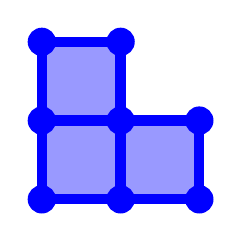
\begin{tikzpicture}[baseline=1cm]
    \foreach \x/\y in {0/0, 0/1, 1/0}{
        \fill[blue!40](\x,\y) rectangle (\x+1,\y+1);
    }
    \foreach \x/\y in {0/0, 0/1, 1/0, 1/1, 0/2, 1/2, 2/0, 2/1}{
        \fill[blue] (\x,\y) circle (1.8mm);
    }
    \foreach \x/\y in {0/0, 0/1, 0/2, 1/0, 1/1}{
    \draw[blue, line width = 1.3mm](\x,\y)--(\x + 1,\y);
    }
    \foreach \x/\y in {0/0, 0/1, 1/0, 1/1, 2/0}{
    \draw[blue, line width = 1.3mm](\x,\y)--(\x,\y+1);
    }
\end{tikzpicture}
\quad
=
\qquad
\tikz{\fill[blue] (0,0) circle (1.8mm)}
\qquad
=\sqrt{2}.\label{qdimKW0}
\end{align}
最初の等号は、(ア)、(イ)を繰り返すことで得られます。次の等号は、\tikz{\fill[blue] (0,0) circle (1.8mm)} に割り当てられたEuler相殺項です。拘束条件の方は自動的に満たされます。

対称性欠陥の場合、\ref{sec:symmetrydefect}章で見たように、可縮な円周の期待値は1であることが分かりますから\footnote{厳密にはアノマリーがあるような対称性の場合、1にならないこともあります。しかし、その場合でも絶対値は1になります。}可縮な円周の期待値が$\sqrt{2}$であるKW欠陥は対称性欠陥ではないということになります。このことから\kyou{KW欠陥は非可逆対称性の欠陥の例であることが分かります。}

\section{対称性の構造}
ここでは、対称性の構造について見ていきます。2次元Ising模型のKW欠陥を含むような非可逆対称性を表すのに便利な数学的構造はフュージョン圏と呼ばれています。フュージョン圏の物理学者向けの分かりやすい解説は\cite{Bhardwaj:2017xup}にあります。

ここでは、数学的な説明というよりは、場の理論の演算子関係式、あるいはWard-Takahashi 恒等式として説明したいと思います。
また、有限群の対称性もフュージョン圏で表されるので、その場合にどうなるかも説明ます。
フュージョン圏の主な構造は次の3つです。
\begin{itemize}
  \item 足し算:相関関数にした後で足し算をします。
  \item フュージョン則:有限群の対称性の場合には、掛け算の構造になります。
  \item F記号:有限群の対称性の場合には、アノマリーの構造になります。
\end{itemize}
これらについて、有限群の場合とIsing模型の対称性(\kyou{Ising圏}と呼ぶことにします)を例にして説明します。

\subsection{足し算}

2次元の次元1のトポロジカル欠陥の種類を圏論の言葉を借りて「対象」(object)と呼ぶことにします。対象と、欠陥が入っている幾何学的な線を考えると具体的なトポロジカル欠陥になります。対象を表す記号を$a$と書き、2次元時空内の連結な端のない線を$C$として欠陥を$L_{a}(C)$と書くことにします。例えば、群の対称性欠陥の場合、群の元は対象です。

実は、群の対称性の場合でも、群の元だけが対象というわけではありません。(群の掛け算以外に)群の形式的な足し算を考えることができます。
\begin{align}
  L_{a+b}(C):=L_{a}(C)+L_{b}(C)\label{objectplus}
\end{align}
と定義します(\ref{sec:remarks}節で説明した演算子関係式の意味です)。

ここで、注意深い人は次の点が心配になるかもしれません。\ref{sec:defect}節の最初で説明したように、そもそも欠陥は局所的でなければなりません。この欠陥$L_{a}(C)+L_{b}(C)$は局所的でしょうか?少なくとも局所性は自明ではありません。また、足し算を考えましたが、引き算や複素数倍はどうでしょうか?

実は足し算は次のように考えると局所的であることが分かります。まず、$C$上に系とは結合していないスカラー場の自由度$n=1,2$を置きます。そして$C$に沿った微分$\del_{t}n$が$\del_{t}n=0$とします。この拘束条件は局所的であることに注意してください。$C$は連結としているので$n$の取りうる値は$C$全体で$1$または$C$全体で$2$です。したがって、この欠陥を挿入した分配関数は、挿入しないものの2倍になります。この欠陥は自明な欠陥を2つ足したものと思うことができます。

一般の欠陥の足し算を考える場合には、次のように考えます。上と同様に$C$上に$n=1,2$を導入して$\del_{t}n=0$の拘束条件を考えます。今度はこの$n$と系を結合させます。$n=1$の部分では、欠陥$L_a$となり、$n=2$の場合はとします。$L_a$も$L_b$も局所的な欠陥で、$n$も局所場ですからこれは局所的な結合です。したがって、こうして作った欠陥は局所的です。この欠陥の対象を$a+b$と定義します。分配関数を考えると\eqref{objectplus}の定義と同じものになります。

上の作り方からは引き算は考えられないことに注意してください。非負の整数以外の複素数倍も局所的にすることはできません。\eqref{qdimKW0}で可縮な円周のKW欠陥の期待値を考えましたが、これに勝手に$1/\sqrt{2}$をかけて期待値を$1$にすることは、局所性を破ります。したがって、$\sqrt{2}$には意味があります。

少し言葉について説明します。他の対象の足し算で書けない対象を\kyou{単純対象}(simple object)と言います。単純対象が有限個しかない場合、このフュージョン圏は\kyou{有限生成}(finitely generated)であると言います。定義から有限生成のフュージョン圏の対象はいくつかの単純対象の和で書けます。有限群の対称性の場合、単純対象は群の元です。Ising圏の単純対象は自明対象$1$、spin flip $\eta$、KW欠陥$\Ncal$の3つです。

以降、2次元では有限生成のフュージョン圏のみ考えます。

\subsection{フュージョン則}

2次元空間内で、2つのトポロジカル欠陥を間になにも挟まずにおいたもの

\subsection{F記号}


\section{応用}


\chapter{高次形式対称性}
\section{高次形式対称性の定義}
\section{格子ゲージ理論の中心対称性}
\section{背景ゲージ場その1}
\section{背景ゲージ場その2:単体コホモロジー}
\section{自発的対称性の破れ}


\chapter{高次元の非可逆対称性}
\section{高次形式対称性のゲージ化}
\section{4次元\texorpdfstring{\Ztwo}{Z2}格子ゲージ理論}
\section{Maxwell理論}

\bibliographystyle{utphys}
\bibliography{ref}
\end{document}
